\input{setup.tex}

% Режим шаблона (должен быть включен один из трех)
\ВКРtrue
%\Практикаtrue
%\Курсоваяtrue

\newcommand{\Дисциплина}{<<Проектирование и архитектура программных систем>>} % для курсовой
\newcommand{\КодСпециальности}{09.03.04} % Курсовая
\newcommand{\Специальность}{Программная инженерия} % Курсовая
\newcommand{\Тема}{Веб-приложение <<Социомаркет для владельцев} % ВКР Курсовая TODO ВКР
\newcommand{\ТемаВтораяСтрока}{домашних животных>>} % TODO ВКР
\newcommand{\ГдеПроводитсяПрактика}{Юго-Западном государственном университете} % для практики
\newcommand{\РуководительПрактПредпр}{Куркина А. В.} % для практики
\newcommand{\ДолжнРуководительПрактПредпр}{директор} % для практики
\newcommand{\РуководительПрактУнивер}{Чаплыгин А. А.} % для практики
\newcommand{\ДолжнРуководительПрактУнивер}{к.т.н. доцент} % для практики
\newcommand{\Автор}{А. Г. Петраков}
\newcommand{\АвторРод}{Петракова А.Г.}
\newcommand{\АвторПолностьюРод}{Петракова Александра Геннадьевича} % для практики
\newcommand{\Шифр}{19-06-0276}
\newcommand{\Курс}{4} % для практики
\newcommand{\Группа}{ПО-92з}
\newcommand{\Руководитель}{Е. И. Аникина} % для ВКР и курсовой
\newcommand{\Нормоконтроль}{А. А. Чаплыгин} % для ВКР
\newcommand{\ЗавКаф}{А. В. Малышев} % для ВКР
\newcommand{\ДатаПриказа}{«24» ноября 2023~г.} % для ВКР
\newcommand{\НомерПриказа}{5470-с} % для ВКР
\newcommand{\СрокПредоставления}{«25» января 2024~г.} % для ВКР, курсового TODO ВКР

\begin{document}
\maketitle
\ifПрактика{}\else{
   \newpage
\begin{center}
\large\textbf{Минобрнауки России}

\large\textbf{Юго-Западный государственный университет}
\vskip 1em
\normalsize{Кафедра программной инженерии}
\vskip 1em
\ifВКР{
        \begin{flushright}
        \begin{tabular}{p{.4\textwidth}}
        \centrow УТВЕРЖДАЮ: \\
        \centrow Заведующий кафедрой \\
        \hrulefill \\
        \setarstrut{\footnotesize}
        \centrow\footnotesize{(подпись, инициалы, фамилия)}\\
        \restorearstrut
        «\underline{\hspace{1cm}}»
        \underline{\hspace{3cm}}
        20\underline{\hspace{1cm}} г.\\
        \end{tabular}
        \end{flushright}
        }\fi
\end{center}
\vspace{1em}
  \begin{center}
  \large
\ifВКР{
ЗАДАНИЕ НА ВЫПУСКНУЮ КВАЛИФИКАЦИОННУЮ РАБОТУ
  ПО ПРОГРАММЕ БАКАЛАВРИАТА}
  \else
ЗАДАНИЕ НА КУРСОВУЮ РАБОТУ (ПРОЕКТ)
\fi
\normalsize
  \end{center}
\vspace{1em}
{\parindent0pt
  Студента \АвторРод, шифр\ \Шифр, группа \Группа
  
1. Тема «\Тема\ \ТемаВтораяСтрока»
\ifВКР{
утверждена приказом ректора ЮЗГУ от \ДатаПриказа\ № \НомерПриказа
}\fi.

2. Срок предоставления работы к защите \СрокПредоставления

3. Исходные данные для создания программной системы:

3.1. Перечень решаемых задач:}

\renewcommand\labelenumi{\theenumi)}

\begin{enumerate}
\item Разработка и создание каталогов с категориями карточек на сайте, обеспечивающих удобный доступ к информации и услугам для владельцев домашних животных;
\item Разработка клиентской части веб-приложения, фокусирующейся на пользовательском интерфейсе и взаимодействии с пользователями;
\item Реализация формы для создания и управления карточкой услуги, упрощающей процесс взаимодействия с сайтом;
\item Создание эффективного и удобного механизма поиска по каталогам и карточкам услуг;
\item Разработка механизма взаимодействия между пользователями сайта, способствующего обмену информацией и опытом;
\item Разработка и развертывание инфраструктуры веб-приложения, включая базу данных на удаленном сервере, для обеспечения его стабильной и надежной работы;
\item Разработка серверной части веб-приложения, обеспечивающей обработку запросов и управление данными;
\item Создание REST API для эффективного взаимодействия между клиентской и серверной частями приложения;
\item Разработка базы данных, обеспечивающей хранение и управление данными веб-приложения.
\end{enumerate}

{\parindent0pt
  3.2. Входные данные и требуемые результаты для программы:}

\begin{enumerate}
\item Входными данными для программной системы являются: данные пользователей и данные о питомцах;
данные о продуктах и услугах, данные для авторизации пользователей и поставщиков услуг;
запросы на поиск продуктов (товаров и услуг);
данные для создания, редактирования и управления карточками продуктов (товаров и услуг);
\item Выходными данными для программной системы являются: данные пользователей и поставщиков услуг с соответствующей информацией;
данные со списками карточек продуктов (товаров и услуг);
данные результатов поиска, соответствующие заданным фильтрам;
обновленные и отредактированные карточки продуктов (товаров и услуг).
\end{enumerate}

{\parindent0pt

  4. Содержание работы (по разделам):
  
  4.1. Введение
  
  4.1. Анализ предметной области
  
4.2. Техническое задание: основание для разработки, назначение разработки,
требования к программной системе, требования к оформлению документации.

4.3. Технический проект: общие сведения о программной системе, проект
данных программной системы, проектирование архитектуры программной системы, проектирование пользовательского интерфейса программной системы.

4.4. Рабочий проект: спецификация компонентов и классов программной системы, тестирование программной системы, сборка компонентов программной системы.

4.5. Заключение

4.6. Список использованных источников

5. Перечень графического материала:

\списокПлакатов

\vskip 2em
\begin{tabular}{p{6.8cm}C{3.8cm}C{4.8cm}}
Руководитель \ifВКР{ВКР}\else работы (проекта) \fi & \lhrulefill{\fill} & \fillcenter\Руководитель\\
\setarstrut{\footnotesize}
& \footnotesize{(подпись, дата)} & \footnotesize{(инициалы, фамилия)}\\
\restorearstrut
Задание принял к исполнению & \lhrulefill{\fill} & \fillcenter\Автор\\
\setarstrut{\footnotesize}
& \footnotesize{(подпись, дата)} & \footnotesize{(инициалы, фамилия)}\\
\restorearstrut
\end{tabular}
}

\renewcommand\labelenumi{\theenumi.}

   \abstract{РЕФЕРАТ}

Объем работы равен \formbytotal{lastpage}{страниц}{е}{ам}{ам}. Работа содержит \formbytotal{figurecnt}{иллюстраци}{ю}{и}{й}, \formbytotal{tablecnt}{таблиц}{у}{ы}{}, \arabic{bibcount} библиографических источников и \formbytotal{числоПлакатов}{лист}{}{а}{ов} графического материала. Количество приложений – 3. Графический материал представлен в приложении А. Фрагменты исходного кода серверной части приложения представлены в приложении Б. Фрагменты исходного кода клиентской части приложения представлены в приложении В.

Перечень ключевых слов: веб-приложение, домашние животные, социальная сеть, социомаркет.

Объектом разработки является веб-приложение <<Социомаркет для владельцев домашних животных>>, представляющее собой платформу, на которой владельцы домашних животных могут находить и предлагать различные услуги и товары.

Целью работы является создания веб-приложения с интуитивно понятным интерфейсом и полезными функциями.

Серверная часть системы разработана на .NET Core, а клиентская часть на Angular. База данных системы построена на PostgreSQL, что обеспечивает её надежность и эффективность.

Веб-приложение оптимизировано для работы в любом браузере на компьютере или мобильном устройстве пользователя.

Для размещения программы на стороне сервера необходим компьютер с операционной системой Windows 10, процессор с тактовой частотой не ниже 1.6 ГГц, ОЗУ 1024 Мб. Для обеспечения стабильной работы базы данных необходимо место на жестком диске 1 ГБ или больше. Для работы серверной части приложения также потребуется установка программной платформы .NET 6.0, а для клиентской части -\- Node.js v12.11.0.

Состояние системы: веб-приложение находится на стадии внедрения и доступно для использования всеми заинтересованными сторонами.

\selectlanguage{english}
\abstract{ABSTRACT}
  
The volume of work is \formbytotal{lastpage}{page}{}{s}{s}. The work contains \formbytotal{figurecnt}{illustration}{}{s}{s}, \formbytotal{tablecnt}{table}{}{s}{s}, \arabic{bibcount} bibliographic sources and \formbytotal{числоПлакатов}{sheet}{}{s}{s} of graphic material. The number of applications is 3. The graphic material is presented in annex A. Fragments of the source code of the server part of the application are presented in Appendix B. Fragments of the source code of the client part of the application are presented in Appendix C.

List of keywords: web application, pets, social network, social marketplace.

The object of development is the web application <<Sociomarket for pet owners>>, which is a platform on which pet owners can find and offer various services and products.

The goal of the work is to create a convenient and functional platform.

The server part of the system is developed based on .NET Core, and the client part is based on Angular. The system database is built on PostgreSQL, which ensures its reliability and efficiency.

To operate the application on the user side, you need a mobile device or computer with Internet access and a browser installed. The application is optimized to work in both modern and older versions of browsers and does not require significant hardware resources.

To host the program on the server side, you need a computer with the Windows 10 operating system, a processor with a clock frequency of at least 1.6 GHz, and 1024 MB of RAM. To ensure stable operation of the database, a hard disk space of 1 GB or more is required. To operate the server part of the application, you will also need to install the .NET 6.0 software platform, and for the client part -\- Node.js v12.11.0.

System Status: The web application is in the implementation stage and is available for use by all interested parties.

\selectlanguage{russian}
}\fi
\tableofcontents
\section*{ОБОЗНАЧЕНИЯ И СОКРАШЕНИЯ}

БД -\- база данных.

СУБД -\- система управления базами данных.

ООП -\- объектно-ориентиронное программирование.

EF Core -\- Entity Framework Core, система управления объектно-реляционным отображением для .NET Core.

ORM -\- Object-Relational Mapping, технология программирования, позволяющая использовать базы данных с объектно-ориентированным подходом.

Angular -\- фреймворк для разработки веб-приложений.

HTML -\- HyperText Markup Language, язык гипертекстовой разметки.

JavaScript -\- язык программирования для веб-разработки.

SCSS -\- Sassy CSS, препроцессор, расширяющий возможности CSS.

UI -\- User Interface, пользовательский интерфейс.

REST API -\- Representational State Transfer Application Programming Interface, интерфейс программирования приложений, использующий архитектурный стиль REST.

CRUD -\- Create, Read, Update, Delete, основные операции для работы с данными.

MVC -\- Model-View-Controller, архитектурный шаблон проектирования.
\ifПрактика{}\else{\section*{ВВЕДЕНИЕ}
\addcontentsline{toc}{section}{ВВЕДЕНИЕ}

Цифровизация и инновации в сфере услуг для домашних животных значительно расширяют горизонты для предпринимателей и пользователей. Настоящая дипломная работа посвящена разработке веб-приложения «Социомаркет для владельцев домашних животных», направленного на улучшение доступности и качества услуг для владельцев домашних животных.

\emph{Цель настоящей работы} -\- разработка веб-приложения, объединяющего владельцев домашних животных и предоставляющих услуги для них. 

Для достижения цели настоящей работы были поставлены \emph{следующие задачи:}

\begin{itemize}
    \item провести анализ предметной области;
    \item разработать пользовательский интерфейс клиентской части приложения;
    \item спроектировать архитектуру и разработать серверную часть приложения;
    \item реализовать клиент-серверное взаимодействие частей приложений.
\end{itemize}

\emph{Структура и объем работы.} Данный отчет представляет собой выпускную квалификационную работу, которая включает в себя введение, четыре основных раздела, заключение, список использованных источников и два приложения. Общий объем текста этой работы составляет \formbytotal{page}{страниц}{у}{ы}{}.

\emph{Во введении} определена цель и поставлены задачи, описана структура работы и представлено краткое содержание каждого из разделов.

\emph{В первом разделе} подробно рассмотрены актуальные аспекты рынка услуг для животных, рассмотрено воздействие цифровой трансформации на обслуживание, а также проанализированы инновационные тенденции и технологии, связанные с предоставлением услуг временного содержания животных.

\emph{Во втором разделе} сформулированы основные требования к разработке веб-приложения. В нем содержатся цели и задачи проекта, а также требования пользователя к интерфейсу. Кроме того, данный раздел охватывает различные функциональные аспекты и обсуждает архитектуру системы.

\emph{В третьем разделе} объясняется выбор используемых технологий проектирования, таких как .NET Core, Entity Framework Core, PostgreSQL и Angular. Также в этом разделе осуществляется проектирование пользовательского интерфейса и предоставление описания классов системы.

\emph{В четвертом разделе} данной работы представлен подробный список классов и их методов, которые были использованы в процессе разработки сайта. Кроме того, в этом разделе проводится детальное тестирование разработанного веб-сайта, с целью проверки его функциональности и стабильности.

\emph{В заключении} преподносятся основные выводы и результаты, полученные в ходе разработки проекта.

В приложении А представлен графический материал.
В приложении Б представлены фрагменты исходного кода серверной части приложения. 
В приложении В представлены фрагменты исходного кода клиентской части приложения. }\fi
```latex
\section{Анализ предметной области}

\subsection{Обзор рынка услуг для животных}

\subsubsection{Обзор современного рынка временного содержания}

Рынок временного содержания домашних животных представляет собой значительный сегмент в сфере услуг для животных. Его размер продолжает расти, особенно в контексте урбанизации и изменений в образе жизни людей. Этот рынок включает услуги по уходу за животными во время отсутствия владельцев, предлагая решения от традиционных гостиниц для животных до индивидуальных нянь.

Анализ предметной области для веб-приложения <<Социомаркет>>, платформы для владельцев домашних животных, начинается с общего обзора рынка временного содержания. Этот рынок, который является значительным сегментом в сфере услуг для животных, продолжает расти, учитывая урбанизацию и изменения в образе жизни людей. Он включает в себя услуги по уходу за животными в период отсутствия владельцев, от традиционных гостиниц для животных до услуг индивидуальных нянь.

Среди текущих тенденций на этом рынке выделяются индивидуализация услуг, которая подразумевает учет уникальных потребностей каждого животного, а также внедрение цифровых технологий. Эти технологии облегчают бронирование услуг, позволяют отслеживать состояние животных и обеспечивают прозрачность услуг. Также наблюдается повышенный интерес к экологически устойчивым и этическим практикам в уходе за животными.

Глобальный рынок услуг для домашних животных, включая временное содержание, продолжает расти, оцениваясь в 216 миллиардов долларов в 2020 году с прогнозом достижения 350 миллиардов к 2027 году, с годовым ростом 6,1\%​​. В России, по данным ВЦИОМ, 68\% семей имеют домашних животных. Рынок услуг разделен на хирургию, диагностические тесты и мониторинг физического здоровья​​. Ключевые российские игроки на рынке включают такие компании, как <<Доктор Зоо>>, <<Зоогигиена>>, и <<Ветбиосфера>>, предлагающие широкий спектр услуг от груминга до ветеринарной помощи.

\subsubsection{Изменения в спросе и предложении услуг}

Рассмотрим влияние изменений в спросе и предложении услуг. Для начала, важно понимать, что данный рынок динамичен и подвержен влиянию различных факторов, включая социальные изменения, экономические тренды и технологические инновации.

Экономические тренды – изменения в потребитель

ских расходах, динамика цен, глобализация рынков, и эволюция цифровой коммерции. Понимание этих трендов помогает компаниям прогнозировать спрос, адаптироваться к меняющимся условиям рынка и разрабатывать долгосрочные стратегии. Экономическая ситуация влияет на расходы владельцев домашних животных. В периоды экономического спада может наблюдаться сокращение расходов на определенные услуги, однако уход за здоровьем и благополучием животных остается приоритетным. Интересно, что кризисные периоды могут стимулировать спрос на более доступные и инновационные услуги, что открывает новые возможности для предпринимателей.

Влияние социальных изменений в результате привносят внедрение новых технологий или значительное улучшение существующих технологий для создания новых или улучшенных продуктов и услуг. Современное общество демонстрирует растущую привязанность к домашним животным, что способствует увеличению спроса на разнообразные услуги, от ветеринарной помощи до досуга и обучения. Эта тенденция также стимулирует рост сегмента услуг по уходу за животными на дому, таких как выгул собак и уход за животными во время отпусков владельцев.

\subsubsection{Роль цифровых платформ}

Цифровые платформы в России, такие как <<Петбук>> и <<Петмир>>, играют ключевую роль в соединении владельцев домашних животных с провайдерами услуг. Аналогичные платформы активно развиваются и в азиатских странах, обеспечивая удобство бронирования и прозрачность цен.

Цифровые платформы радикально изменили поведение потребителей. Владельцы домашних животных теперь имеют доступ к широкому спектру услуг и продуктов онлайн. Это включает в себя возможность сравнивать цены, читать отзывы и общаться с другими владельцами животных. Такое взаимодействие влияет на принятие решений и способствует формированию онлайн-сообществ.

Цифровые платформы предлагают различные бизнес-модели, включая прямые продажи, подписку, фриемиум-модели и комиссионные сборы. Для веб-приложения <<Социомаркет>>, ключевым может стать вопрос о том, как монетизировать свою пользовательскую базу, не уменьшая при этом удовлетворенность пользователей.

Инновации играют критическую роль в развитии цифровых платформ. Использование искусственного интеллекта для персонализации предложений, блокчейн для обеспечения прозрачности и безопасности транзакций, и интеграция с социальными сетями для повышения вовлеченности пользователей – все это актуальные темы для веб-приложений, направленных на владельцев домашних животных.

Цифровые платформы обеспечивают непосредственное взаимодействие с пользователем. Это позволяет собирать обратную связь и быстро реагировать на предпочтения и проблемы пользователей. Для <<Социомаркета>> важно создать эффективный канал обратной связи и использовать его для улучшения пользовательского опыта.
\subsection{Цифровизация в обслуживании}
\subsubsection{Переход к онлайн-бронированию}

Онлайн-бронирование стало стандартом в индустрии услуг для домашних животных в России и Азии, предлагая удобство и доступность услуг.
\subsubsection{Особенности взаимодействия через цифровые каналы}

Цифровые каналы позволяют предоставлять более персонализированные услуги и улучшают коммуникацию между владельцами животных и провайдерами услуг.
\subsubsection{Поведение пользователей в онлайн-сервисах}

Пользователи ценят удобство, безопасность и прозрачность при использовании онлайн-сервисов. Они ожидают высокого уровня обслуживания и надежности, а также возможности быстро решать возникающие вопросы.

Пользовательский опыт и отзывы. Пользовательский опыт охватывает все аспекты взаимодействия пользователя с компанией, ее услугами и продуктами. Целью является создание положительного и эффективного опыта для пользователя. Отзывы пользователей же представляют собой обратную связь от клиентов, которая помогает компаниям улучшать их продукты и услуги. В контексте веб-приложений, это означает интуитивно понятные интерфейсы, быструю и эффективную поддержку, а также регулярное обновление функционала на основе отзывов пользователей. В эпоху цифровизации роль отзывов потребителей и их влияние на репутацию брендов усиливаются. Предприятиям важно уделять внимание отзывам клиентов и стремиться к улучшению пользовательского опыта, чтобы привлекать и удерживать клиентов.

Индивидуальный подход и персонализация – создание продуктов или услуг, адаптированных к индивидуальным потребностям и предпочтениям каждого пользователя. В сфере цифровых платформ это может включать в себя персонализированные рекомендации, настройки интерфейса и контента, а также предложения, основанные на предыдущем поведении и предпочтениях пользователя. Персонализация улучшает пользовательский опыт и повышает лояльность клиентов. Современные потребители ожидают, что услуги будут максимально адаптированы к их нуждам и предпочтениям. Это может включать персонализированные программы питания для животных, индивидуальные тренировки или даже персонализированные аксессуары.

Ключевую роль на рынке играют социальные маркетплейсы, которые соединяют владельцев домашних животных с поставщиками услуг. Важную роль играют и инновационные стартапы, предлагающие уникальные решения, включая мобильные приложения и интегрированные сервисы.

Для глубокого исследования этого рынка необходимо учитывать разработку интуитивно понятного интерфейса, интеграцию с социальными сетями для возможности делиться отзывами, анализ потребностей рынка через опросы и исследования. Также важно сотрудничество с ветеринарами и другими экспертами для гарантии качества предоставляемых услуг. Этот анализ может быть расширен в более обширный документ, который будет включать детализированные исследования каждого из этих аспектов, а также исследование конкурентов, маркетинговую стратегию и план развития.
\subsection{Инновации и технологические тренды}
\subsubsection{Новейшие технологии в отрасли}

Современный рынок услуг для домашних животных переживает технологический бум. Основные направления включают разработку мобильных приложений для управления ветеринарными услугами, интеграцию Интернета Вещей для мониторинга состояния животных, и создание платформ для эффективного поиска услуг по уходу за питомцами. Эти технологии способствуют улучшению качества ухода и обеспечивают более глубокое взаимодействие между владельцами животных и сервисами. Примерами компаний, внедряющих эти технологии, являются Butternut Box и Creature Comforts, предлагающие инновационные подходы в уходе за животными и ветеринарные услуги соответственно.
\subsubsection{Влияние инноваций на качество и доступность услуг}

Инновации значительно повлияли на качество и доступность услуг для домашних животных. Онлайн-платформы и мобильные приложения упрощают доступ к информации и услугам, что особенно важно в условиях глобализации и урбанизации. Улучшение качества услуг достигается за счет применения передовых технологий, таких как телемедицина, что позволяет владельцам животных получать консультации специалистов на расстоянии. Компании, такие как Scrumbles и Mon Véto, демонстрируют эти тенденции, предлагая продукты питания и ветеринарные услуги на новом технологическом уровне.
\subsubsection{Примеры успешных технологических проектов}

Примеры успешных проектов включают платформы для поиска надежных нянь для животных, системы удаленного мониторинга здоровья питомцев, и приложения для социального взаимодействия владельцев животных. Эти проекты демонстрируют, как технологии могут улучшить жизнь животных и облегчить уход за ними. Выдающиеся примеры включают Micron Agritech, разработчика портативных тестов для обнаружения паразитарных инфекций у скота, и Digitail, облачное ветеринарное программное обеспечение.
\subsection{Развитие услуг временного содержания}
\subsubsection{Анализ потребностей клиентов}

Потребности клиентов в области временного содержания домашних животных включают надежность, безопасность и индивидуальный подход к уходу. Владельцы животных ищут сервисы, которые могут гарантировать качественный уход и поддержку. Важным фактором является также удобство бронирования услуг и прозрачность в отношении условий содержания. Компании, такие как PetSmart Inc. и Dogtopia Enterprises, отражают эти потребности, предоставляя широкий спектр услуг с акцентом на безопасность и комфорт.
\subsubsection{Технологические решения для улучшения сервиса}

Для улучшения качества услуг временного содержания используются различные технологические решения. Это включает в себя системы управления данными о питомцах, мобильные приложения для отслеживания состояния животных в реальном времени, и автоматизированные системы для управления бронированиями и обратной связи. Компании Ultra Premium Direct и Japhy являются примерами организаций, внедряющих эти технологии для оптимизации ухода и питания домашних животных.
\subsubsection{Обзор специализированных платформ}

Специализированные платформы предлагают разнообразные услуги, от временного ухода до медицинского обслуживания. Они отличаются удобством использования, наличием обширной базы данных о поставщиках услуг и возможностью обратной связи от пользователей. Такие платформы способствуют повышению доверия и удобства для клиентов. Примерами таких платформ являются Pawz and Company и Paradise 4 Paws, предоставляющие уникальные и индивидуализированные услуги по уходу за животными.
\subsection{Перспективы и направления будущего развития}
\subsubsection{Анализ предстоящих инноваций}

Анализ предстоящих инноваций показывает, что ключевые направления включают развитие искусственного интеллекта и машинного обучения для более точного анализа потребностей животных и их владельцев, а также внедрение блокчейн-технологий для повышения безопасности и прозрачности транзакций. Компании, такие как Younikat и Mammaly, демонстрируют эти инновации, фокусируясь на разработке продуктов питания и здоровья животных.
\subsubsection{Внедрение новых технологий}

Внедрение новых технологий включает в себя интеграцию передовых аналитических инструментов для лучшего понимания рынка и потребностей клиентов, а также разработку новых цифровых инструментов для улучшения взаимодействия с клиентами и управления услугами. Примерами таких компаний являются Barkibu, предоставляющая страхование здоровья животных, и Food for Joe, производитель кормов.
\subsubsection{Оценка будущих трендов в отрасли}

Будущие тренды в отрасли включают усиление роли устойчивости и этики в уходе за животными, расширение интернет-сообществ владельцев животных для обмена опытом и информацией, а также развитие индивидуализированных и персонализированных услуг, учитывающих уникальные потребности клиента и бизнеса.
\section{Техническое задание}
\subsection{Основание для разработки}

Полное наименование системы: <<Веб-приложение \textquotedbl Социомаркет для владельцев домашних животных \textquotedbl\ >>.
Основанием для разработки программы является приказ ректора ЮЗГУ от <<24>> ноября 2023 г. №5166-с <<Об утверждении тем выпускных квалификационных работ>>.

\subsection{Цель и назначение разработки}

Веб-приложение <<Социомаркет для владельцев домашних животных>> создается с целью объединения пользователей двух групп: владельцев домашних животных и лиц, предоставляющих услуги для домашних животных. Такими лицами могут являться владельцы интернет-магазинов, предприниматели или такие же пользователи.

Задачами данной разработки являются:
\begin{itemize}
\item создание каталогов с категориями карточек на сайте;
\item разработка клиентской части web-сайта;
\item создание каталогов с категориями карточек на сайте;
\item реализация формы создания и управления карточкой услуги;
\item создание удобного поиска по каталогам карточкам;
\item реализация взаимодействия между пользователями сайта;
\item разработка и развертывание инфраструктуры web-сайта и его базы данных на удаленном сервере;
\item разработка серверной части web-сайта;
\item разработка REST API для взаимодействия клиентской и серверной частей;
\item разработка базы данных.
\end{itemize}

Задачей разработки серверной части так же является следования принципам, описанным в работе Марка Прайса <<C\# 9 и .NET 5. Разработка и оптимизация>>~\cite{mark_price}.

\subsection{Требования пользователя к интерфейсу web-сайта}

Сайт должен включать в себя:
\begin{itemize}
    \item авторизацию;
    \item навигацию по разделам;
    \item разделение доступа к функционалу сайта для пользователя и лица предоставляющего услуги;
    \item поиск по пользователям и их товарам или услугам.
\end{itemize}


\subsection{Требования к программной системе веб-приложения <<Социомаркет>>}
\subsubsection{Требования к данным программной системы}
Система должна уметь эффективно обрабатывать данные пользователей, включая личную информацию, данные о питомцах, информацию о продуктах (товары и услуги). Необходимо обеспечить конфиденциальность и безопасность этих данных.
На рисунке ~\ref{bd:image} представлена концептуальная модель данных программной системы в виде UML-диаграммы сущность-связь.

\begin{figure}[ht]
\centering
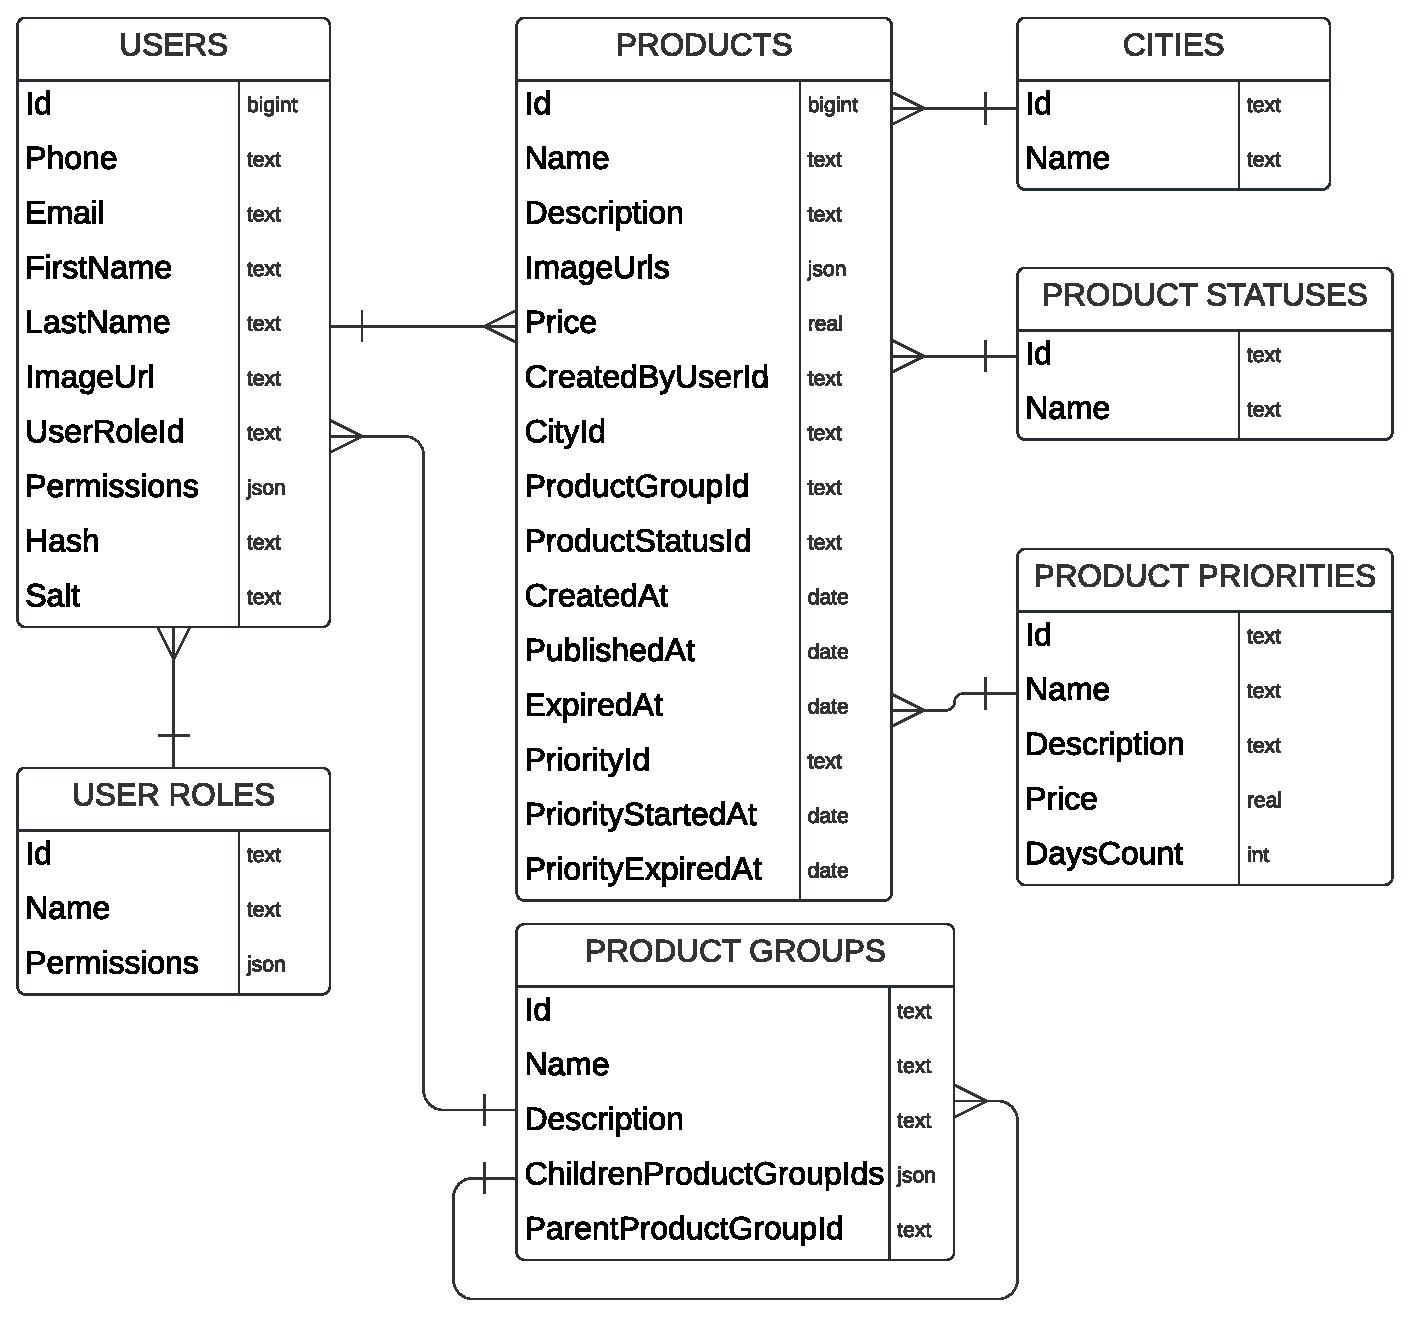
\includegraphics[width=1\linewidth]{bd}
\caption{Концептуальная модель данных}
\label{bd:image}
\end{figure}

В приведенной на рисунке ~\ref{bd:image} диаграмме сущность-связь представлены сущности и атрибуты, которые будут использоваться в программной системе.

Данные программной системы должны быть организованы таким образом, что бы не разделять на 2 отдельные группы пользователей и лиц, предоставляющих услуги. Отличие между пользователями должно быть записано в атрибуте <<UserRole>> сущности <<User>>. Таким образом, в программной системе будет только одна сущность <<User>>, которая будет иметь атрибут <<UserRole>> со значениями <<SITTER>> и <<OWNER>>.
При проектировании модели данных так же необходимо ущесто то, что сущность <<Product>> представляет собой продукт, который может быть как товаром, так и услугой. Для этого не требуется никаких дополнительных атрибутов, так как сущность <<Product>> становится товаром или услугой в зависисмости от названия и описания карточки продукта.

\subsubsection{Функциональные требования к программной системе}
В разрабатываемой программно-информационной системе должно быть предусмотрено наличие двух классов пользователей: владельцев домашних животных и лиц, предоставляющих услуги или товары для них.

\subsubsection{Архитектура системы} 
Серверная часть веб-приложения <<Социомаркет>> разработана на .NET Core, что отражает современные подходы в разработке программного обеспечения, описанные в <<C\# 9 и .NET 5. Разработка и оптимизация>>~\cite{mark_price}. Клиентская часть, реализованная на Angular, взаимодействует с сервером через REST API. База данных построена на PostgreSQL и соответствует рекомендациям и методикам, изложенным в документации PostgreSQL~\cite{postgresql}.

\subsubsection{Вариант использования <<Авторизация пользователя>>} 
Пользователи входят в систему, используя свой логин и пароль. Предусмотрена возможность восстановления пароля через электронную почту.

\subsubsection{Вариант использования <<Авторизация лица предоставляющего услуги>>}
Поставщики услуг и товаров регистрируются в системе, предоставляя специфическую информацию о предлагаемых услугах или товарах.

\subsubsection{Вариант использования <<Поиск>>} 
Пользователи могут искать продукты которые могут быть как товарами так и услугами, используя ключевые слова и фильтры для уточнения результатов. LINQ-запросы для выполнения поисковых операций.

\subsubsection{Вариант использования <<Просмотр каталогов карточек с товарами и услугами>>}
Пользователи могут просматривать карточки продуктов (товаров и услуг) в каталоге. Каждая карточка содержит информацию о товаре или услуге, включая описание, цену, фотографии и отзывы. Карточки можно фильтровать по категориям или тегам.

\subsubsection{Вариант использования <<Управление своими карточками>>}
Поставщики услуг и товаров могут создавать, редактировать и удалять свои карточки в каталоге. Это включает добавление описаний, цен, фотографий и другой релевантной информации.

\subsubsection{Вариант использования <<Инициировать обмен контактами между пользователями>>} 
Возможность отправить запрос на социальные сети другого пользователя для дальнейшего общения и сотрудничества.

\subsubsection{Вариант использования <<Редактирование профиля пользователя>>}
Пользователи могут редактировать свои личные данные, контактную информацию, а также настройки уведомлений и конфиденциальности.

\subsubsection{Вариант использования <<Просмотр профилей поставщиков услуг>>}
Пользователи могут просматривать профили поставщиков, включая описание услуг, фотографии и отзывы клиентов.

\subsubsection{Вариант использования <<Мобильная версия приложения>>}
Мобильная версия приложения обеспечивает удобство использования на смартфонах и планшетах, адаптируя интерфейс под мобильные устройства.

\subsubsection{Диаграмма прецедентов}
На рисунке ~\ref{people:image} представлена диаграмма прецедентов.

\begin{figure}[ht]
\centering
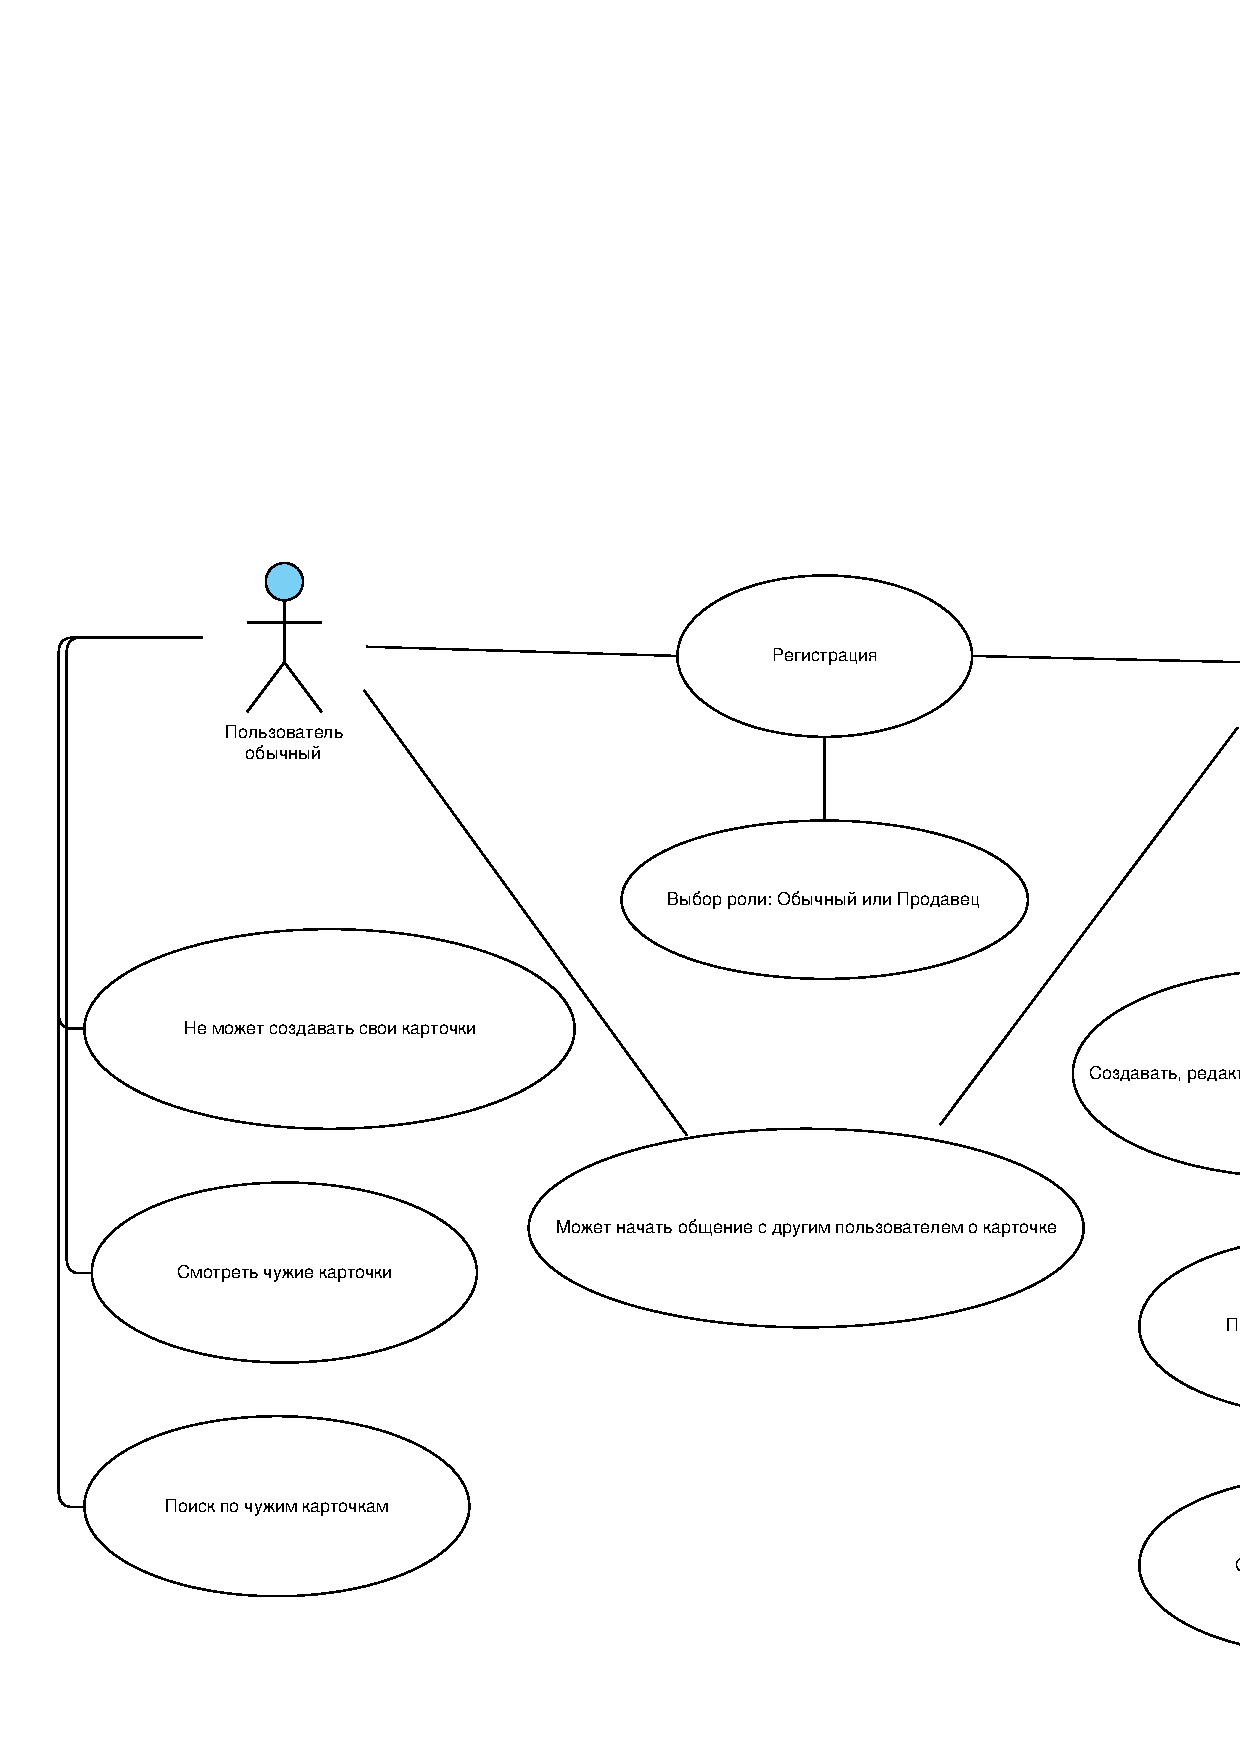
\includegraphics[width=1\linewidth]{people}
\caption{Диаграмма прецедентов}
\label{people:image}
\end{figure}

\subsection{Требования пользователя к интерфейсу приложения}
Интерфейс должен быть интуитивно понятным, удобным для пользователя, с четкой навигацией и адаптивным дизайном, подходящим для различных устройств. Принципы разработки интерфейса и адаптивного дизайна основаны на спецификациях HTML и CSS, как указано в <<Спецификация CSS>>~\cite{cssspecs} и <<Спецификация HTML>>~\cite{htmlbook}.
При проектировании интерфейса следует отказаться от диалоговых окон для крупных элементов сайта. То есть регистрация, поиск, результат поиска - все они будут на отдельных страницах, а не внутри диалоговых окон.

\subsection{Нефункциональные требования к программной системе}

\subsubsection{Требования к надежности}
В процессе работы серверной части программной системы возможны следующие аварийные ситуации:
\begin{enumerate}
\item Потеря доступа к сети Интернет;
\item Аварийное отключение электропитания;
\item Сбой операционной системы сервера.
\end{enumerate}

Для минимизации вероятности возникновения аварийных событий серверные компоненты программной системы должны быть размещены на выделенных серверах в дата-центрах хостинг-провайдеров, прошедших сертификацию и имеющих гарантию SLA>99,8\%. Операционная системадолжна получать регулярные накопительные обновления.

\subsubsection{Требования к безопасности}
Наличие механизма проверки целостности приложения путем использования криптографических функций, основанных на подписи пакета программы. Коммуникация с сервером по защищенному протоколу.

Требования к безопасности серверной части программной системы:
\begin{enumerate}
\item Регулярные обновления компонентов безопасности операционной системы;
\item Автоматическое обновление HTTPS-сертификатов;
\item Доступ к серверу должен осуществляться без разглашения IP-адреса целевой машины в целях предотвращения возможных атак типа DDoS;
\item Запросы к серверу должны предварительно обрабатываться на одельной машине с запущенным экземпляром сервера Nginx для контроля количества запросов и логирования обращений к серверу;
\item Правилами брандмауэра операционной системы основного сервера должно быть разрешено подключение к порту сервера только с IP-адреса промежуточной машины.
\end{enumerate}

Требования к безопасности клиентской части программной системы:
\begin{enumerate}
\item Поддержка современных браузеров и операционных систем, обеспечивающая стабильную и безопасную работу на различных платформах;
\item Использование технологий адаптивной верстки приложения;
\item Реализация защиты от XSS и CSRF атак, предотвращающая нежелательное вмешательство в работу приложения;
\item Регулярное обновление компонентов системы для предотвращения уязвимостей, связанных с устаревшим программным обеспечением.
\end{enumerate}

\subsubsection{Требования к программному обеспечению}
Для реализации программной системы должны быть использованы следующие языки программирования:
С\# -\- серверная часть приложения;
Type-script -\- клиентская часть приложения;
SQL -\- язык структурированных запросов к базе данных.

Для работы клиентской части приложения требуется ОС Android 5.0 или более поздняя версия или Windows 7 или более поздняя версия с установленным браузером Google Chrome.
Для работы серверных компонентов требуется ОС Windows 7 или Macos 12.0 или Ubuntu 16.0 или более поздняя версия c установленной СУБД PostgreSQL, .NET CORE 6.0, .NET SDK 6.0.

\subsubsection{Требования к аппаратному обеспечению}
Для сервера необходим центральный процессор с количеством ядер от 6 и выше с частотой ядра от 2.4 ГГц. Объем оперативной памяти – 32 Гб. Требование к скорости интернет-соединения – 100 Мбит/c и выше.

\subsection{Требования к оформлению документации}
Требования к стадиям разработки программ и программной документации для вычислительных машин, комплексов и систем независимо от их назначения и области применения, этапам и содержанию работ устанавливаются ГОСТ 19.102–77.
Программная документация должна включать в себя:

\begin{enumerate}
\item Анализ предметной области;
\item Техническое задание;
\item Технический проект;
\item Рабочий проект.
\end{enumerate}

\section{Технический проект}

\subsection{Общая характеристика организации решения задачи}
Обсуждение методологии разработки, включая Agile подходы, планирование спринтов и процессы контроля качества.

\subsection{Обоснование выбора технологий проектирования}
\subsubsection{.NET Core}
Обоснование выбора .NET Core для серверной разработки: производительность, масштабируемость и кросс-платформенность.
Начиная с версии .NET core 6.0, которая была выбрана для разработки, поддерживается работа с админ-панелью "из коробки", что позволяет сэкономить ресурсы на ращработки панели администратора.
\subsubsection{Entity Framework Core}
Entity Framework Core является ORM (Object-Relational Mapping) для .NET Core. Он позволяет работать с базами данных, используя объектно-ориентированный подход. Entity Framework Core позволяет работать с различными СУБД, в том числе с PostgreSQL, которая была выбрана для разработки.
\subsubsection{Angular}
Angular является самым строгим и требовательным к архитектуре среди других Frontend библиотек. Такие свойства Angular делают его идеальным инструментом для разработки сложных масштабируемых приложений. Мощные инструменты для создания интерактивных интерфейсов и легкость интеграции с REST API.

\subsection{Проектирование пользовательского интерфейса}

На основании требований к пользовательскому интерфейсу, представленных в пункте 2.3 технического задания, был разработан графический интерфейс мобильного приложения. Для создания пользовательского интерфейса используется Frontend приложение на библиотеке Angular с применением разметки HTML, языка программирования JavaScript и SCSS.
Разработанный интерфейс ориентирован на обеспечение легкости в использовании и интуитивного понимания функционала приложения, предоставляя пользователю гладкое и эффективное взаимодействие с приложением.

\begin{enumerate}
    \item \textbf{Поиск}: Реализация функции поиска на основе поля \textit{ProductName} из класса \textit{Product}, \textit{Price}, \textit{Weight}, и \textit{ProductGroupId} класса \textit{Product}.
    \item \textbf{Отображение результатов поиска}: Эффективное представление списка товаров, включая \textit{ImageUrl}, \textit{ProductName}, информацию о \textit{Category} и \textit{Price}.
    \item \textbf{Детали товара}: Дополнительная информация о товаре, включая его \textit{Category} и \textit{Weight}.
    \item \textbf{Навигация по приложению}: Элементы навигации, такие как кнопка возврата к началу списка и индикаторы категорий.
\end{enumerate}

\begin{figure}[h!]
    \includegraphics[width=0.82\linewidth]{interface-search.png}
    \caption{модели интерфейса <<Поиск>> и <<Навигация по приложению>>}
    \label{fig:search}
\end{figure}

Процесс регистрации пользователя в приложении максимально упрощен и включает следующие шаги:
\begin{enumerate}
    \item Пользователь выбирает опцию <<Регистрация>> на главном экране.
    \item Заполняются основные поля: электронная почта, имя пользователя и пароль.
    \item Пользователь должен подтвердить свой адрес электронной почты через полученное письмо со ссылкой для подтверждения.
    \item После подтверждения электронной почты, пользователь может ввести дополнительную информацию в свой профиль: фотографию, контактные данные и предпочтения в приложении.
    \item На последнем этапе пользователь принимает условия пользования и политику конфиденциальности, после чего регистрация завершается.
\end{enumerate}

Регистрация дог-ситтеров предполагает прохождение дополнительных этапов для верификации и предоставления информации о предоставляемых услугах:
\begin{enumerate}
    \item Потенциальный дог-ситтер начинает регистрацию с выбора соответствующего пункта в приложении.
    \item Вводятся личные данные, включая полное имя, адрес проживания и номер телефона.
    \item Запрашивается информация о предыдущем опыте работы с животными и наличии соответствующих рекомендаций.
    \item Дог-ситтер должен пройти онлайн-курс по уходу за животными и предоставить сертификат о его окончании.
    \item Предоставляется информация об услугах, включая доступные даты и временные рамки, а также устанавливаются тарифы.
    \item Профиль дог-ситтера отправляется на проверку. После одобрения администрацией профиль становится доступным для поиска и выбора пользователями.
\end{enumerate}

% На рисунке ~\ref{register:image} представлены модели интерфейса регистации <<Пользователя>> и <<Дог-ситтера>>.

\begin{figure}[h!]
    \includegraphics[width=0.82\linewidth]{interface-register.png}
    \caption{Модели интерфейса регистрации "Пользователя" и "Дог-ситтера"}
    \label{fig:register}
\end{figure}

% \begin{figure}[ht]interface-register.png
% \includegraphics[width=1\linewidth]{register}
% \caption{модели интерфейса регистации <<Пользователя>> и <<Дог-ситтера>>}
% \label{register:image}
% \end{figure}
% \subsection{Диаграмма компонентов и схема обмена данными между файлами компонента}

% Диаграмма компонентов описывает особенности физического представления разрабатываемой системы. Она позволяет определить архитектуру системы, установив зависимости между программными компонентами, в роли которых может выступать как исходный, так и исполняемый код. Основными графическими элементами диаграммы компонентов являются компоненты, интерфейсы, а также зависимости между ними. На рисунке \ref{comp:image} изображена диаграмма компонентов для проектируемой системы. Она включает в себя сервер с операционной системой, на которой установлена система управления содержимым, включающая в себя базу данных и интерфейс. Помимо этого на диаграмме изображен клиентский компьютер с операционной системой, на которой установлен браузер.

% \begin{figure}[ht]
% \center{\includegraphics[width=1\linewidth]{comp}}
% \caption{Диаграмма компонентов}
% \label{comp:image}
% \end{figure}

% Любой компонент должен быть вызван в сценарии страницы web-сайта. Web-страница передает данные компоненту в момент вызова последнего.
%
% На рисунке \ref{data:image} представлена схема обмена данными между сценариями компонента при вызове компонента на странице сайта.
%
% \begin{figure}[ht]
% \center{\includegraphics[width=1\linewidth]{data}}
% \caption{Диаграмма компонентов}
% \label{data:image}
% \end{figure}
%
% При вызове компонента в сценарии web-страницы указываются значения параметров компонента, которые далее посредством массива \$arParams передаются в сценарий файла component.php.
%
% В сценарии файла component.php посредством метода \linebreak IncludeComponentTemplate класса CBitrixComponent происходит вызов одного из шаблонов компонента. Id шаблона также определяется в сценарии страницы web-приложения и неявно для разработчика передается указанный выше метод. Подключается сценарий файла template.php одного из шаблонов, в который передается, возможно, измененный в сценарии component.php массив \$arParams и, также, сформированный в сценарии component.php массив \$arResult. Оба этих массива доступны также и в файле result\_modifier.php, который подключается перед подключением файла template.php.
%
% Работа компонента заканчивается в момент завершения работы сценария файла component.php, т.е. возможно выполнить действия уже после подключения шаблона. Однако, если массив \$arResult будет изменен в сценарии шаблона, в сценарий файла компонента component.php измененные данные переданы не будут.

\subsection{Диаграмма размещения}

Диаграмма размещения (рис.~\ref{place:image}) отражает физические взаимосвязи между программными и аппаратными компонентами системы.

\begin{figure}[ht]
\center{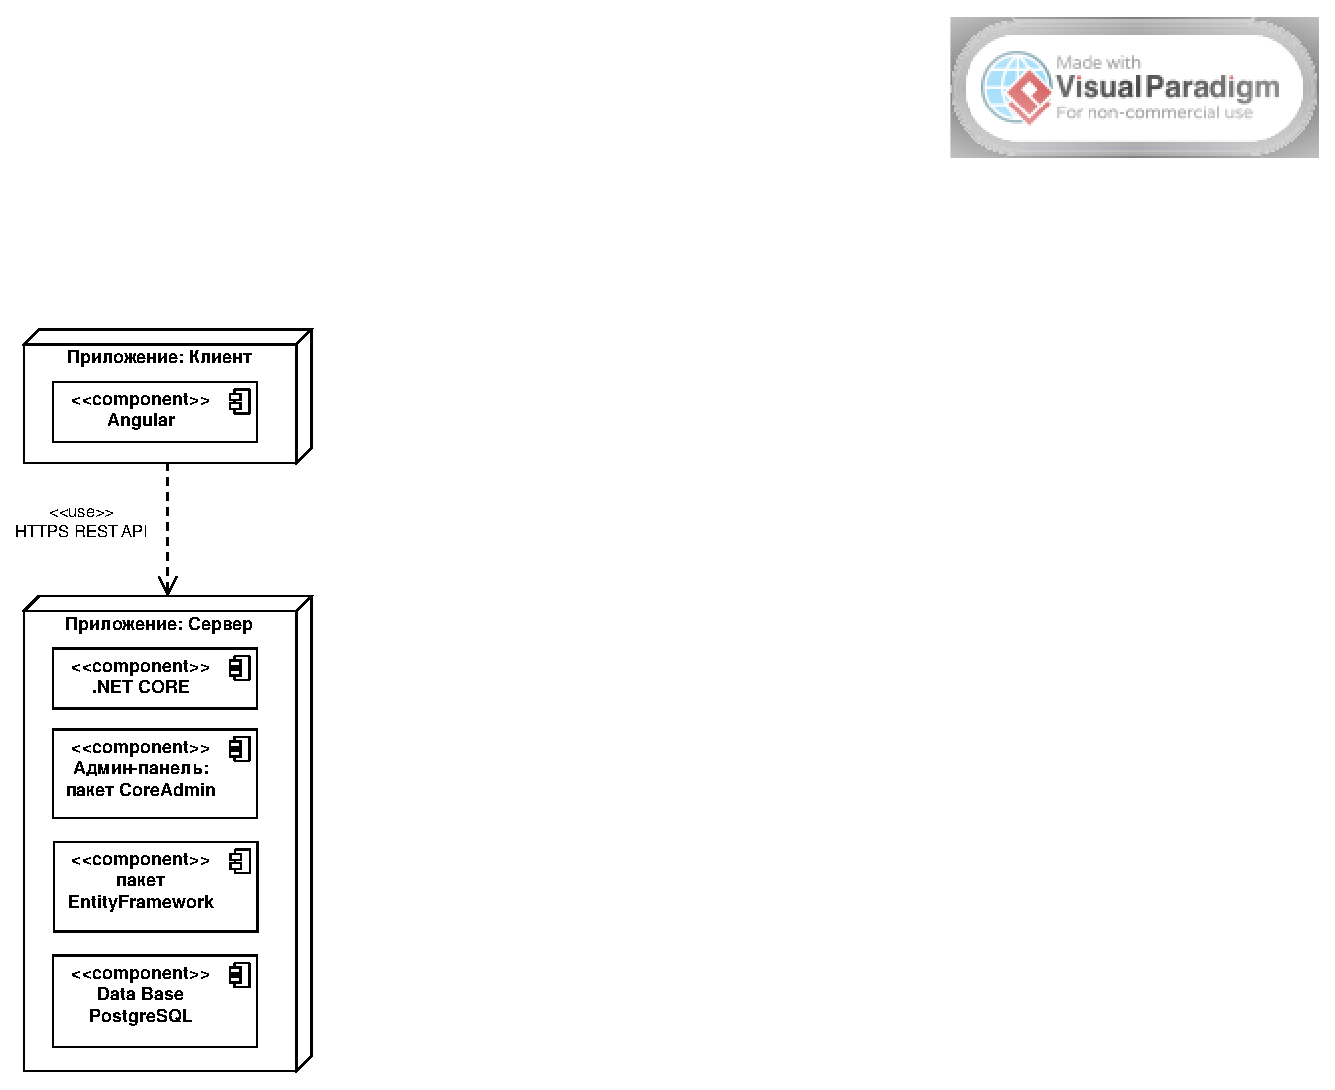
\includegraphics[width=1\linewidth]{client-server.eps}}
\caption{Диаграмма размещения}
\label{place:image}
\end{figure}

Она является хорошим средством для показа маршрутов перемещения объектов и компонентов в распределенной системе.

\subsection{Описание классов системы}

\subsubsection{Описание классов серверной части}

\begin{itemize}
    \item <<UserBase>> служит основой для всех пользовательских данных, предоставляя общие поля, такие как <<Phone>>, <<Email>>, <<FirstName>>, <<LastName>>, и т.д.
    \item <<UserRegistrationData>> расширяет <<UserBase>>, добавляя специфичное для регистрации поле <<Password>>.
    \item <<UserLoginData>> используется для процесса входа в систему, содержа только <<Email>> и <<Password>>.
    \item <<UserLoginResponseData>> и <<UserView>> расширяют <<UserBase>>, добавляя уникальный идентификатор <<Id>>, а <<UserLoginResponseData>> также включает <<AccessToken>> для аутентификации.
    \item <<User>> является полным представлением пользователя, включающим безопасность (через <<Hash>> и <<Salt>>) и <<Id>>.
\end{itemize}

% Таблица для UserBase
\begin{xltabular}{\textwidth}{|l|l|p{1.7cm}|X|}
    \caption{Атрибуты сущности "UserBase"}\\ \hline
    Поле & Тип & Обяза\-тельное & Описание \\ \hline
    Phone & String & false & Телефонный номер пользователя \\ \hline
    Email & String & false & Электронная почта пользователя \\ \hline
    FirstName & String & false & Имя пользователя \\ \hline
    LastName & String & false & Фамилия пользователя \\ \hline
    ImageUrl & String & false & URL изображения пользователя \\ \hline
    Telegram & String & false & Telegram пользователя \\ \hline
    Website & String & false & Веб-сайт пользователя \\ \hline
\end{xltabular}

% Таблица для UserRegistrationData
\begin{xltabular}{\textwidth}{|l|l|p{1.7cm}|X|}
    \caption{Атрибуты сущности "UserRegistrationData"}\\ \hline
    Поле & Тип & Обяза\-тельное & Описание \\ \hline
    % Здесь перечислены атрибуты из UserBase
    Password & String & true & Пароль пользователя \\ \hline
\end{xltabular}

% Таблица для UserLoginData
\begin{xltabular}{\textwidth}{|l|l|p{1.7cm}|X|}
    \caption{Атрибуты сущности "UserLoginData"}\\ \hline
    Поле & Тип & Обяза\-тельное & Описание \\ \hline
    Email & String & true & Электронная почта пользователя для входа \\ \hline
    Password & String & true & Пароль пользователя для входа \\ \hline
\end{xltabular}

% Таблица для UserLoginResponseData
\begin{xltabular}{\textwidth}{|l|l|p{1.7cm}|X|}
    \caption{Атрибуты сущности "UserLoginResponseData"}\\ \hline
    Поле & Тип & Обяза\-тельное & Описание \\ \hline
    % Здесь перечислены атрибуты из UserBase
    Id & Long & true & Уникальный идентификатор пользователя \\ \hline
    AccessToken & String & true & Токен доступа пользователя \\ \hline
\end{xltabular}

% Таблица для UserView
\begin{xltabular}{\textwidth}{|l|l|p{1.7cm}|X|}
    \caption{Атрибуты сущности "UserView"}\\ \hline
    Поле & Тип & Обяза\-тельное & Описание \\ \hline
    % Здесь перечислены атрибуты из UserBase
    Id & Long & true & Уникальный идентификатор пользователя \\ \hline
\end{xltabular}

% Таблица для User
\begin{xltabular}{\textwidth}{|l|l|p{1.7cm}|X|}
    \caption{Атрибуты сущности "User"}\\ \hline
    Поле & Тип & Обяза\-тельное & Описание \\ \hline
    % Здесь перечислены атрибуты из UserBase
    Id & Long & true & Уникальный идентификатор пользователя \\ \hline
    Hash & String & true & Хэш пользователя \\ \hline
    Salt & String & true & Соль для хэша пароля пользователя \\ \hline
\end{xltabular}

\begin{itemize}
    \item <<Product>>, наследующийся от <<Short>>, описывает основную информацию о продукте, такую как <<ImageUrl>>, <<ProductGroupId>>, <<Price>>, <<Weight>>, и <<CreatedByUserId>>, указывающий на пользователя, создавшего продукт.
    \item <<ProductView>> расширяет <<Product>>, добавляя <<CreatedByUser>>, который является экземпляром <<UserView>>. Это позволяет получать не только идентификационную информацию о создателе продукта, но и более детальные данные пользователя.
\end{itemize}

% Таблица для Product
\begin{xltabular}{\textwidth}{|l|l|p{1.7cm}|X|}
    \caption{Атрибуты сущности "Product"}\\ \hline
    Поле & Тип & Обяза\-тельное & Описание \\ \hline
    % Здесь перечислены атрибуты из Short
    ImageUrl & String & false & URL изображения продукта \\ \hline
    ProductGroupId & Long & true & Идентификатор группы продуктов \\ \hline
    Price & Float & true & Цена продукта \\ \hline
    Weight & Integer & true & Вес продукта \\ \hline
    CreatedByUserId & Long & true & Идентификатор пользователя, создавшего продукт \\ \hline
\end{xltabular}

% Таблица для ProductView
\begin{xltabular}{\textwidth}{|l|l|p{1.7cm}|X|}
    \caption{Атрибуты сущности "ProductView"}\\ \hline
    Поле & Тип & Обяза\-тельное & Описание \\ \hline
    % Здесь перечислены атрибуты из Product
    CreatedByUser & UserView & true & Пользователь, создавший продукт \\ \hline
\end{xltabular}


% По аналогии создаются таблицы для UserLoginData, UserLoginResponseData, UserView, User

% В таблице \ref{ssevsws:table} приведен пример использования пакета xltabular с автоматическим расчетом ширины столбца.
%
% \begin{xltabular}{\textwidth}{|c|X|X|}
% 	\caption{Сравнение протоколов SSE и WebSocket\label{ssevsws:table}}\\ \hline
% 	~  & \centrow  SSE & \centrow WebSocket \\ \hline
% 	\endfirsthead
% 	\continuecaption{Продолжение таблицы \ref{ssevsws:table}}
% 	~ & \centrow SSE & \centrow WebSocket \\ \hline
% 	\finishhead
% 	Направленность &
% 	Однонаправленный, полудуплексный: данные посылает только сервер &
% 	Двунаправленный, полнодуплексный: и сервер, и клиент могут обмениваться сообщениями \\ \hline
% 	Соединение  & HTTP & WS \\ \hline
% 	Тип данных & Только текст & Бинарные и текстовые данные \\ \hline
% 	Доп. возможности & Встроенный механизм идентификаторов событий и переподключения & Переподключение и идентификация события реализуются на стороне приложения
% \end{xltabular}

% Проанализировав требования, можно выделить шесть основных сущностей:
% \begin{itemize}
% \item "<Новости">;
% \item "<Продукция">;
% \item "<Услуги">.
% \end{itemize}
%
% В состав сущности "<Новости"> можно включить атрибуты, представленные в таблице \ref{news:table}.
%
% \begin{xltabular}{\textwidth}{|l|l|p{1.7cm}|X|}
% 	\caption{Атрибуты сущности "<Новости">\label{news:table}}\\ \hline
% 	\centrow Поле & \centrow Тип & \centrow Обяза\-тельное & \centrow Описание \\ \hline
% 	\thead{1} & \thead{2} & \centrow 3 & \centrow 4 \\ \hline
% 	\endfirsthead
% 	\continuecaption{Продолжение таблицы \ref{news:table}}
% 	\thead{1} & \thead{2} & \centrow 3 & \centrow 4 \\ \hline
% 	\finishhead
% 	\_id & ObjectId & true & Уникальный идентификатор \\ \hline
% 	head & String & true & Заголовок новости \\ \hline
% 	short & String & false & Аннотация к новости \\ \hline
% 	createdAt & Date & true & Время создания новости \\ \hline
% 	author & String & false & Автор новости \\ \hline
% 	content & String & true & Текст новости \\ \hline
% 	views & Integer & true & Количество просмотров новости зарегистрированными пользователями
% \end{xltabular}
%
% Пример использования различных типов столбцов представлен в таблице \ref{prod:table}. Рекомендуется использовать пакет xltabular для создания таблиц.
%
% \begin{xltabular}{\textwidth}{|R|C{2.5cm}|l|T|}
% 	\caption{Атрибуты  сущности "<Новости разметки в LaTeX"> с использованием различных типов столбцов и многострочным заголовком\label{prod:table}}\\ \hline
% 	\centrow Поле & \centrow Тип & \centrow Обязательное & \centrow Описание \\ \hline
% 	\centrow 1 & \centrow 2 & \thead{3} & \centrow 4 \\ \hline
% 	\endfirsthead
% 	\continuecaption{Продолжение таблицы \ref{prod:table}}
% 	\centrow 1 & \centrow 2 & \thead{3} & \centrow 4 \\ \hline
% 	\finishhead
% 	\_id & ObjectId & true & Уникальный идентификатор \\ \hline
% 	head & String & true & Заголовок новости \\ \hline
% 	short & String & false & Аннотация к новости \\ \hline
% 	createdAt & Date & true & Время создания новости \\ \hline
% 	author & String & false & Автор новости \\ \hline
% 	content & String & true & Текст новости \\ \hline
% 	views & Integer & true & Количество просмотров новости зарегистрированными пользователями
% \end{xltabular}

В системе предусмотрен внутренний механизм связи между разделами и элементами информационных блоков, поэтому введения дополнительных идентификаторов при реализации связей между сущностями не предполагается.

Экземпляры сущностей реализуются в информационных блоках посредством элементов, атрибуты сущности – посредством полей и свойств элемента. 

\ifПрактика{}\else{
   \section{Рабочий проект}
\subsection{Описание REST API приложения}

Можно выделить следующий перечень HTTP-методов, использованных при разработке веб-приложения и доступных для использования клиентской частью приложения. Описание этих методов предоставлены в виде аблиц с уменьшенным межстрочным интервалом:
\begin{itemize}
    \item описания методов для работы с городами (таблица \ref{city:table});
    \item описание методов для работы с карточками товаров и услуг (таблица \ref{product:table});
    \item описание методов для работы с типами товаров и услуг (таблица \ref{type:table});
    \item описание методов для работы с данными пользователя (таблица \ref{data:table}).
\end{itemize}

\renewcommand{\arraystretch}{0.8} % уменьшение расстояний до сетки таблицы

\begin{xltabular}{\textwidth}{|X|p{2.5cm}|>{\setlength{\baselineskip}{0.7\baselineskip}}p{4.85cm}|>{\setlength{\baselineskip}{0.7\baselineskip}}p{4.85cm}|}
    \caption{Описания методов для работы с городами\label{city:table}}\\
    \hline \centrow \setlength{\baselineskip}{0.7\baselineskip} HTTP-метод & \centrow \setlength{\baselineskip}{0.7\baselineskip} Описание & \centrow Входные параметры & \centrow Пример JSON ответа \\
    \hline \centrow 1 & \centrow 2 & \centrow 3 & \centrow 4\\ \hline
    \endfirsthead
    \caption*{Продолжение таблицы \ref{city:table}}\\
    \hline \centrow 1 & \centrow 2 & \centrow 3 & \centrow 4\\ \hline
    \finishhead
    GET /api /City  & Список всех городов City в БД & Нет & [ \{ 
      id: 0, 
      name: <<string>>, 
      description: <<string>> 
        \} 
      ] \\
\end{xltabular}
    

\begin{xltabular}{\textwidth}{|X|p{2.5cm}|>{\setlength{\baselineskip}{0.7\baselineskip}}p{4.85cm}|>{\setlength{\baselineskip}{0.7\baselineskip}}p{4.85cm}|}
    \caption{Описание методов для работы с карточками товаров и услуг\label{product:table}}\\
    \hline \centrow \setlength{\baselineskip}{0.7\baselineskip} HTTP-метод & \centrow \setlength{\baselineskip}{0.7\baselineskip} Описание & \centrow Входные параметры & \centrow Пример JSON ответа \\
    \hline \centrow 1 & \centrow 2 & \centrow 3 & \centrow 4\\ \hline
    \endfirsthead
    \caption*{Продолжение таблицы \ref{product:table}}\\
    \hline \centrow 1 & \centrow 2 & \centrow 3 & \centrow 4\\ \hline
    \finishhead
    GET /api /Product  & Список всех карточек Product & Нет & [
        \{
      id: 0,
      name: <<string>>,
      description: <<string>>,
      imageUrl: <<string>>,
      price: 0,
      createdByUserId: 0,
      cityId: 0,
      productGroupId: 0,
      productStatusId: 0,
      createdAt: <<2024-01-20>>,
      publishedAt: <<2024-01-20>>,
      expiredAt: <<2024-01-20>>,
      priorityId: 0,
      priorityStartedAt: <<2024-01-20>>,
      priorityExpiredAt: <<2024-01-20>>,
      createdByUser: \{
        phone: <<string>>,
        email: <<string>>,
        firstName: <<string>>,
        lastName: <<string>>,
        imageUrl: <<string>>,
        telegram: <<string>>,
        website: <<string>>,
        userRoleId: <<string>>,
        permissions: <<string>>,
        id: 0
          \}
        \}
      ]\\
\hline POST /api /Product  & Создать новый Product & Body: \{
id: 0,
name: <<string>>,
description: <<string>>,
imageUrl: <<string>>,
price: 0,
createdByUserId: 0,
cityId: 0,
productGroupId: 0,
productStatusId: 0,
createdAt: <<2024-01-20>>,
publishedAt: <<2024-01-20>>,
expiredAt: <<2024-01-20>>,
priorityId: 0,
priorityStartedAt: <<2024-01-20>>,
priorityExpiredAt: <<2024-01-20>>,
createdByUser: \{
  phone: <<string>>,
  email: <<string>>,
  firstName: <<string>>,
  lastName: <<string>>,
  imageUrl: <<string>>,
  telegram: <<string>>,
  website: <<string>>,
  userRoleId: <<string>>,
  permissions: <<string>>,
  id: 0
    \}
  \} & \{
id: 0,
name: <<string>>,
description: <<string>>,
imageUrl: <<string>>,
price: 0,
createdByUserId: 0,
cityId: 0,
productGroupId: 0,
productStatusId: 0,
createdAt: <<2024-01-20>>,
publishedAt: <<2024-01-20>>,
expiredAt: <<2024-01-20>>,
priorityId: 0,
priorityStartedAt: <<2024-01-20>>,
priorityExpiredAt: <<2024-01-20>>
  \}\\
\hline GET /api /Product /\{id\} & Получить выбранный Product по его id & Нет & \{
id: 0,
name: <<string>>,
description: <<string>>,
imageUrl: <<string>>,
price: 0,
createdByUserId: 0,
cityId: 0,
productGroupId: 0,
productStatusId: 0,
createdAt: <<2024-01-20>>,
publishedAt: <<2024-01-20>>,
expiredAt: <<2024-01-20>>,
priorityId: 0,
priorityStartedAt: <<2024-01-20>>,
priorityExpiredAt: <<2024-01-20>>
  \}\\
\hline PUT /api /Product /\{id\} & Обновить существующий Product & Body: \{
id: 0,
name: <<string>>,
description: <<string>>,
imageUrl: <<string>>,
price: 0,
createdByUserId: 0,
cityId: 0,
productGroupId: 0,
productStatusId: 0,
createdAt: <<2024-01-20>>,
publishedAt: <<2024-01-20>>,
expiredAt: <<2024-01-20>>,
priorityId: 0,
priorityStartedAt: <<2024-01-20>>,
priorityExpiredAt: <<2024-01-20>>,
createdByUser: \{
  phone: <<string>>,
  email: <<string>>,
  firstName: <<string>>,
  lastName: <<string>>,
  imageUrl: <<string>>,
  telegram: <<string>>,
  website: <<string>>,
  userRoleId: <<string>>,
  permissions: <<string>>,
  id: 0
    \}
  \} & \{
id: 0,
name: <<string>>,
description: <<string>>,
imageUrl: <<string>>,
price: 0,
createdByUserId: 0,
cityId: 0,
productGroupId: 0,
productStatusId: 0,
createdAt: <<2024-01-20>>,
publishedAt: <<2024-01-20>>,
expiredAt: <<2024-01-20>>,
priorityId: 0,
priorityStartedAt: <<2024-01-20>>,
priorityExpiredAt: <<2024-01-20>>
  \}\\
\hline DELETE /api /Product /\{id\} & Удалить Product по его id & Нет & Нет\\
\hline GET /api /Product /filter & Получить отфильтрованный список существующих продуктов & Query parameters: cityId: integer, productGroupId: integer, publishedAtFrom: string, expiredAtTo: string. & [
    \{
  id: 0,
  name: <<string>>,
  description: <<string>>,
  imageUrl: <<string>>,
  price: 0,
  createdByUserId: 0,
  cityId: 0,
  productGroupId: 0,
  productStatusId: 0,
  createdAt: <<2024-01-20>>,
  publishedAt: <<2024-01-20>>,
  expiredAt: <<2024-01-20>>,
  priorityId: 0,
  priorityStartedAt: <<2024-01-20>>,
  priorityExpiredAt: <<2024-01-20>>
    \}
  ]\\
\end{xltabular}

\begin{xltabular}{\textwidth}{|X|p{2.5cm}|>{\setlength{\baselineskip}{0.7\baselineskip}}p{4.85cm}|>{\setlength{\baselineskip}{0.7\baselineskip}}p{4.85cm}|}
    \caption{Описание методов для работы с типами товаров и услуг\label{type:table}}\\
    \hline \centrow \setlength{\baselineskip}{0.7\baselineskip} HTTP-метод & \centrow \setlength{\baselineskip}{0.7\baselineskip} Описание & \centrow Входные параметры & \centrow JSON ответ \\
    \hline \centrow 1 & \centrow 2 & \centrow 3 & \centrow 4\\ \hline
    \endfirsthead
    \caption*{Продолжение таблицы \ref{type:table}}\\
    \hline \centrow 1 & \centrow 2 & \centrow 3 & \centrow 4\\ \hline
    \finishhead
    GET /api /ProductGtoup  & Список всех типов товаров и услуг ProductGroup в БД & Нет & [
        \{
      id: 0,
      name: <<string>>,
      description: <<string>>,
      type: 0,
      childrenProductGroupIds: [
            0
          ],
      parentProductGroupId: 0
        \}
      ]\\
      \hline POST /api /ProductGtoup  & Создать новый ProductGtoup & Body: [
        \{
      id: 0,
      name: <<string>>,
      description: <<string>>,
      type: 0,
      childrenProductGroupIds: [
            0
          ],
      parentProductGroupId: 0
        \}
      ] & [
        \{
      id: 0,
      name: <<string>>,
      description: <<string>>,
      type: 0,
      childrenProductGroupIds: [
            0
          ],
      parentProductGroupId: 0
        \}
      ] \\
\end{xltabular}

\begin{xltabular}{\textwidth}{|X|p{4.85cm}|>{\setlength{\baselineskip}{0.7\baselineskip}}p{2.5cm}|>{\setlength{\baselineskip}{0.7\baselineskip}}p{4.85cm}|}
    \caption{Описание методов для работы с данными пользователя\label{data:table}}\\
    \hline \centrow \setlength{\baselineskip}{0.7\baselineskip} HTTP-метод & \centrow \setlength{\baselineskip}{0.7\baselineskip} Описание & \centrow Входные параметры & \centrow JSON ответ \\
    \hline \centrow 1 & \centrow 2 & \centrow 3 & \centrow 4\\ \hline
    \endfirsthead
    \caption*{Продолжение таблицы \ref{data:table}}\\
    \hline \centrow 1 & \centrow 2 & \centrow 3 & \centrow 4\\ \hline
    \finishhead
    GET /api /User /{id} & Получить данные существующего пользователя User по его id & Нет & \{
    phone: <<string>>,
    email: <<string>>,
    firstName: <<string>>,
    lastName: <<string>>,
    imageUrl: <<string>>,
    telegram: <<string>>,
    website: <<string>>,
    userRoleId: <<string>>,
    permissions: <<string>>,
    id: 0
      \}\\
      \hline POST /api /User /create & Создать нового пользователя User & Body: \{
    phone: <<string>>,
    email: <<string>>,
    firstName: <<string>>,
    lastName: <<string>>,
    imageUrl: <<string>>,
    telegram: <<string>>,
    website: <<string>>,
    userRoleId: <<string>>,
    permissions: <<string>>,
    password: <<string>>
      \} & \{
    phone: <<string>>,
    email: <<string>>,
    firstName: <<string>>,
    lastName: <<string>>,
    imageUrl: <<string>>,
    telegram: <<string>>,
    website: <<string>>,
    userRoleId: <<string>>,
    permissions: <<string>>,
    id: 0,
    hash: <<string>>,
    salt: <<string>>
      \} \\
      \hline POST /api /User /login & Авторизоваться существующим пользователем User в системе. Авторизоваться -\- сохранить в клиентском приложение значение из поля accessToken & Body: \{
    email: <<string>>,
    password: <<string>>
      \} & \{
    phone: <<string>>,
    email: <<string>>,
    firstName: <<string>>,
    lastName: <<string>>,
    imageUrl: <<string>>,
    telegram: <<string>>,
    website: <<string>>,
    userRoleId: <<string>>,
    permissions: <<string>>,
    id: 0,
    accessToken: <<string>>
      \} \\
\end{xltabular}

\renewcommand{\arraystretch}{1.0} % восстановление сетки

\subsection{Модульное тестирование разработанного приложения}


\section{Структура тестового проекта}
В рамках тестирования программного обеспечения был разработан тестовый проект, структура которого представлена на рисунке \ref{testproject_structure:image}. Данный проект включает в себя модульные тесты для различных компонентов системы. Тестирование моделей и контроллеров позволяет обеспечить надежность и корректность работы программного обеспечения.
В тестовый проект добавлена возможность использовать пространство имен из основного проекта с помощью команды: dotnet add reference ../new_back/new_back.csproj.
Тестовый проект включает в себя следующие ключевые элементы:

\begin{itemize}
  \item \textbf{Models}: Классы, которые представляют модели данных, используемые в тестах.
  \item \textbf{Shared}: Вспомогательные классы и утилиты, используемые в различных тестах.
  \item \textbf{TestResults}: Результаты выполнения тестов.
  \item \textbf{UnitTestShort.cs и UnitTestUserController.cs}: Наборы модульных тестов для проверки соответствующих классов и контроллеров.
\end{itemize}

\begin{figure}[ht]
\centering
\includegraphics[width=0.5\textwidth]{testproject_structure.png}
\caption{Структура тестового проекта}
\label{testproject_structure:image}
\end{figure}

Содержимое файла \textbf{ShortTest.cs} представлено на рисунке \ref{st:image}.

\begin{figure}[!ht]
\lstset{style=sharpc}
\begin{lstlisting}
namespace TestProject.Models
{
    [TestClass]
    public class ShortTest
    {
        public long Id { get; set; }
        public string? Name { get; set; }
        public string? Description { get; set; } = null;
    }
}
\end{lstlisting}
\caption{Содержимое файла \textbf{ShortTest.cs}}
\label{st:image}
\end{figure}

Содержимое файла \textbf{Utils.cs} представлено на рисунке \ref{ut:image}.

\begin{figure}[!ht]
\lstset{style=sharpc}
\begin{lstlisting}
namespace TestProject.Shared
{
    public class Utils
    {
        public static void TestString(string v1, string v2)
        {
            if (v1 == null || v2 == null)
            {
                Assert.Fail();
            }

            Assert.AreEqual(v1, v2);
        }

        public static int GenerateUniqueId()
        {
            Random random = new Random();
            return random.Next(1, 101);
        }
    }
}
\end{lstlisting}
\caption{Содержимое файла \textbf{Utils.cs}}
\label{ut:image}
\end{figure}

Содержимое файла \textbf{Usings.cs} представлено на рисунке \ref{usings:image}.

\begin{figure}[!ht]
\lstset{style=sharpc}
\begin{lstlisting}
global using Microsoft.VisualStudio.TestTools.UnitTesting;
global using System.IO;
global using static System.Math;
global using System.Web;
global using Moq;
global using Microsoft.AspNetCore.Mvc;
\end{lstlisting}
\caption{Содержимое файла \textbf{Usings.cs}}
\label{usings:image}
\end{figure}

Модульные тесты для класса Short, который является базовым классом для большинства моделей в приложении, позволяют проверить корректность логики и поведения этого компонента и исключить возникновение проблем в этом классе и его потомков. Тесты охватывают такие аспекты, как валидация имен и описаний, а также уникальность идентификаторов объектов.
Модульные тесты для класса Short представлены на рисунке \ref{unitshort1:image}.

\begin{figure}[ht]
\lstset{style=sharpc}
\begin{lstlisting}
using TestProject.Shared;
using TestProject.Models;

namespace TestProject
{
    [TestClass]
    public class UnitTestShort
    {
        [TestMethod]
        public void Short_Validate_Name()
        {
            var testValue = "Test Name";
            var testObject = new ShortTest() {
                Name = testValue
            };
            Utils.TestString(testObject.Name, testValue);
        }

        [TestMethod]
        public void Short_Validate_Description()
        {
            var testValue = "Test description";
            var testObject = new ShortTest() {
                Description = testValue
            };
            Utils.TestString(testObject.Description, testValue);
        }

        [TestMethod]
        public void Short_Validate_Id()
        {
            var testObject = new ShortTest();
            long randomId = 0;
            while (randomId == 0)
            {
                randomId = Utils.GenerateUniqueId();
            }
            testObject.Id = randomId;
            Assert.AreNotEqual(0, testObject.Id);
            Assert.AreEqual(randomId, testObject.Id);
        }
    }
}  
\end{lstlisting}
\caption{Модульный тест класса Short}
\label{unitshort1:image}
\end{figure}

Для контроллера UserController, который обрабатывает пользовательские запросы, были разработаны тесты, имитирующие взаимодействие с репозиторием данных. Это позволяет тестировать контроллер в изоляции от реальной базы данных, что упрощает процесс разработки и повышает качество кода.
Модульные тесты для UserController представлено на рисунке \ref{unitcontr1:image}.

\begin{figure}[ht]
\lstset{style=sharpc}
\begin{lstlisting}
global using new_back.Controllers;
global using new_back.Infrastructure;
global using new_back.Models;

namespace TestProject
{
    [TestClass]
    public class UserControllerTests
    {
        private Mock<IUserRepository> _mockRepository;
        private UserController _controller;

        [TestInitialize]
        public void SetUp()
        {
            _mockRepository = new Mock<IUserRepository>();
            _controller = new UserController(_mockRepository.Object);
        }

        [TestMethod]
        public void GetById_UserExists_ReturnsUserView()
        {
            long userId = 1;
            var mockUser = new User { Id = userId, Email = "test@example.com" };
            _mockRepository.Setup(repo => repo.GetById(userId)).Returns(mockUser);

            var result = _controller.GetById(userId);

            Assert.IsNotNull(result);
            Assert.IsInstanceOfType(result.Result, typeof(OkObjectResult));

            var okResult = result.Result as OkObjectResult;
            Assert.IsNotNull(okResult);

            var userViewResult = okResult.Value as UserView;
            Assert.IsNotNull(userViewResult);
            Assert.AreEqual(userId, userViewResult.Id);
            Assert.AreEqual("test@example.com", userViewResult.Email);
        }

        [TestMethod]
        public void GetById_UserDoesNotExist_ReturnsNotFound()
        {
            _mockRepository.Setup(repo => repo.GetById(It.IsAny<long>())).Returns((User)null);

            var result = _controller.GetById(1);

            Assert.IsInstanceOfType(result.Result, typeof(NotFoundResult));
        }
    }
}
\end{lstlisting}
\caption{Модульный тест класса UserController}
\label{unitcontr1:image}
\end{figure}

Разработка тестового проекта является ключевым компонентом в цикле обеспечения качества программного продукта. Она демонстрирует эффективность тестирования и его способность гарантировать надежность функционирования системы. На рисунке \ref{testresult:image} представлены результаты выполнения модульных тестов, подтверждающие успешную проверку всех компонентов системы, что свидетельствует об отсутствии критических ошибок и готовности продукта к дальнейшим этапам разработки и внедрения.

\begin{figure}[ht]
\centering
\includegraphics[width=0.8\textwidth]{testresult.png}
\caption{Результаты выполнения модульных тестов}
\label{testresult:image}
\end{figure}

\subsection{Системное тестирование разработанного web-сайта}

На рисунке \ref{main:image} представлена главная страница сайта «Русатом – Аддитивные технологии».
\newpage % при необходимости можно переносить рисунок на новую страницу
\begin{figure}[H] % H - рисунок обязательно здесь, или переносится, оставляя пустоту
\center{\includegraphics[width=1\linewidth]{main1}}
\center{\includegraphics[width=1\linewidth]{main2}}
\center{\includegraphics[width=1\linewidth]{main3}}
\caption{Главная страница сайта «Русатом – Аддитивные технологии»}
\label{main:image}
\end{figure}

На рисунке \ref{menu:image} представлен динамический вывод заголовков, включающий в себя искомые фразы при поиске фраз.

\begin{figure}[ht]
\center{\includegraphics[width=1\linewidth]{menu}}
\caption{Динамический вывод заголовков}
\label{menu:image}
\end{figure}

На рисунке \ref{enter:image} представлен ввод данных для публикации новости.

\begin{figure}[ht]
\center{\includegraphics[width=1\linewidth]{enter}}
\caption{Ввод данных для публикации очень-очень длинной, интересной и полезной новости}
\label{enter:image}
\end{figure}

   \section*{ЗАКЛЮЧЕНИЕ}
\addcontentsline{toc}{section}{ЗАКЛЮЧЕНИЕ}

Инновации и цифровизация в сфере услуг для домашних животных открывают новые возможности как для предпринимателей, так и для пользователей. Разработка веб-приложения «Социомаркет для владельцев домашних животных» успешно демонстрирует, как современные технологии могут способствовать улучшению качества и доступности услуг.

Основные результаты работы:

\begin{enumerate}
\item Проведен глубокий анализ предметной области, включая текущие тенденции и потребности рынка услуг для домашних животных.
\item Разработан и реализован пользовательский интерфейс веб-приложения, обеспечивающий удобство и эффективность использования.
\item Спроектирована и разработана архитектура серверной части приложения, используя современные технологии, такие как .NET Core, Entity Framework Core, PostgreSQL и Angular.
\item Реализовано клиент-серверное взаимодействие, обеспечивающее надежную и эффективную работу приложения.
\end{enumerate}

Все задачи, поставленные в начале работы, были успешно решены. Разработанное веб-приложение соответствует всем современным требованиям и позволяет пользователям эффективно взаимодействовать в рамках предоставления услуг для домашних животных. Приложение характеризуется высоким уровнем удобства использования и доступности, что делает его важным инструментом на рынке услуг для домашних животных.

Веб-приложение «Социомаркет для владельцев домашних животных» полностью соответствует современным стандартам веб-разработки и может внести значительный вклад в развитие сферы услуг для домашних животных.

}\fi
% \addcontentsline{toc}{section}{СПИСОК ИСПОЛЬЗОВАННЫХ ИСТОЧНИКОВ}
%
% \begin{thebibliography}{9}
%
%     \bibitem{javascript} Фримен, А. Практикум по программированию на JavaScript / А. Фримен. – Москва~: Вильямс, 2013. – 960 с. – ISBN 978-5-8459-1799-7. – Текст~: непосредственный.
%     \bibitem{php} Бретт, М. PHP и MySQL. Исчерпывающее руководство / М. Бретт. – Санкт-Петербург : Питер, 2016. – 544 с. – ISBN 978-5-496-01049-8. – Текст~: непосредственный.
%     \bibitem{css} Веру, Л. Секреты CSS. Идеальные решения ежедневных задач / Л. Веру. – Санкт-Петербург : Питер, 2016. – 336 с. – ISBN 978-5-496-02082-4. – Текст~: непосредственный.
%     \bibitem{mysql}	Гизберт, Д. PHP и MySQL / Д. Гизберт. – Москва~: НТ Пресс, 2013. – 320 с. – ISBN 978-5-477-01174-2. – Текст~: непосредственный.
% 	\bibitem{html5}	Голдстайн, А. HTML5 и CSS3 для всех / А. Голдстайн, Л. Лазарис, Э. Уэйл. – Москва~: Вильямс, 2012. – 368 с. – ISBN 978-5-699-57580-0. – Текст~: непосредственный.
% 	\bibitem{htmlcss}	Дэкетт, Д. HTML и CSS. Разработка и создание веб-сайтов / Д. Дэкетт. – Москва~: Эксмо, 2014. – 480 с. – ISBN 978-5-699-64193-2. – Текст~: непосредственный.
% 	\bibitem{bigbook}	Макфарланд, Д. Большая книга CSS / Д. Макфарланд. – Санкт-Петербург : Питер, 2012. – 560 с. – ISBN 978-5-496-02080-0. – Текст~: непосредственный.
% 	\bibitem{uchiru}	Лоусон, Б. Изучаем HTML5. Библиотека специалиста / Б. Лоусон, Р. Шарп. – Санкт-Петербург : Питер, 2013 – 286 с. – ISBN 978-5-459-01156-2. – Текст~: непосредственный.
% 	\bibitem{chaynik}	Титтел, Э. HTML5 и CSS3 для чайников / Э. Титтел, К. Минник. – Москва~: Вильямс, 2016 – 400 с. – ISBN 978-1-118-65720-1. – Текст~: непосредственный.
% 	\bibitem{22}	Титтел, Э. HTML5 и CSS3 для чайников / Э. Титтел, К. Минник. – Москва~: Вильямс, 2016 – 400 с. – ISBN 978-1-118-65720-1. – Текст~: непосредственный.
% 	\bibitem{1231}	Титтел, Э. HTML5 и CSS3 для чайников / Э. Титтел, К. Минник. – Москва~: Вильямс, 2016 – 400 с. – ISBN 978-1-118-65720-1. – Текст~: непосредственный.
% 	\bibitem{sdf}	Титтел, Э. HTML5 и CSS3 для чайников / Э. Титтел, К. Минник. – Москва~: Вильямс, 2016 – 400 с. – ISBN 978-1-118-65720-1. – Текст~: непосредственный.
% 	\bibitem{servsssds}	Титтел, Э. HTML5 и CSS3 для чайников / Э. Титтел, К. Минник. – Москва~: Вильямс, 2016 – 400 с. – ISBN 978-1-118-65720-1. – Текст~: непосредственный.
% \end{thebibliography}
\addcontentsline{toc}{section}{СПИСОК ИСПОЛЬЗОВАННЫХ ИСТОЧНИКОВ}

\begin{thebibliography}{14}

    \bibitem{yordon} Йордон, Э. Путь камикадзе. Как разработчику программного обеспечения выжить в безнадежном проекте / Эдвард Йордон. – Москва : Лори, 2019. – 256 с.

    \bibitem{averin} Аверин, А.В. Стандартизация и регламентация государственных услуг: российский и зарубежный опыт / А.В. Аверин. – Москва : Урал, 2015. – С. 721-727.

    \bibitem{grinchenko} Гринченко, Н.Н. Проектирование баз данных. СУБД Microsoft Ассе: Учебное пособие для вузов / Н.Н. Гринченко и др. – Москва : РиС, 2013. – 240 с.

    \bibitem{postgresql} Postgresql.org -\- Документация базы данных : сайт. - URL: https://www.postgresql.org/docs/ (дата обращения: 20.05.2022). - Текст : электронный.

    \bibitem{akhrameeva} Ахрамеева, О.В. Российское сервисное государство: теоретические основы и государственная стратегия обеспечения частных и публичных интересов / О.В. Ахрамеева. – Москва : Урал, 2014. – С. 1-28.

    \bibitem{makni} Макни, Дж.К. Проектирование серверной инфраструктуры баз данных Microsoft SQL Server 2005 / Дж.К. Макни. – Москва : Русская редакция, 2008. – 560 с.

    \bibitem{cssspecs} W3C Specifications -\- спецификация CSS: сайт. – URL: https://www.w3.org/Style/CSS/specs.en.html (дата обращения: 20.12.2023). – Текст: электронный.

    \bibitem{htmlbook} HTMLBOOK -\- спецификация НТМL: сайт. - URL: http://htmlbook.ru/html (дата обращения: 10.12.2023). - Текст : электронный.

 	\bibitem{html5}	Голдстайн, А. HTML5 и CSS3 для всех / А. Голдстайн, Л. Лазарис, Э. Уэйл. – Москва~: Вильямс, 2012. – 368 с. – ISBN 978-5-699-57580-0. – Текст~: непосредственный.

    \bibitem{boyko} Бойко И. Объектно-ориентированные СУБД / И. Бойко. – Киев : Высшая школа, 2014.

    \bibitem{kumskova} Кумскова, И.А. Базы данных. Учебник для ССУЗов / И.А. Кумскова. – Москва : КноРус, 2012. – 488 с.

    \bibitem{mark_price} Марк Прайс. C\# 9 и .NET 5. Разработка и оптимизация / Марк Прайс. – Санкт-Петербург : Питер, 2021. – 832 с. – ISBN 978-5-4461-2921-8. – Текст: непосредственный.

    \bibitem{msdn} MSDN -\- сеть разработчиков Microsoft [Электронный ресурс]. URL: https://msdn.microsoft.com.

    \bibitem{stackoverflow} StackOverflow -\- сайт вопросов и ответов для программистов [Электронный ресурс]. URL: https://ru.stackoverflow.com/.

    \bibitem{freeman} Фримен, Э. Изучаем Angular: Руководство по созданию приложений на Angular / Эрик Фримен, Элизабет Робсон. – Москва: Эксмо, 2018. – 720 с. – ISBN 978-5-699-98165-6.

    \bibitem{troelsen} Троелсен, Э. Язык программирования C\# 7 и платформы .NET и .NET Core / Эндрю Троелсен, Филип Джепикс. – Москва: Вильямс, 2018. – 1456 с. – ISBN 978-5-8459-2114-9.

    \bibitem{freedman} Фридман, Д. Методы исследования рынков / Дэвид Фридман, Сэм Либерман. – Москва: Альпина Паблишер, 2016. – 560 с. – ISBN 978-5-9614-5403-5.

    \bibitem{riccardi} Риккарди, Дж. ASP.NET Core 6: Современное развитие веб-приложений на C\# / Джейсон Риккарди. – Москва: ДМК Пресс, 2022. – 512 с. – ISBN 978-5-97060-837-9.

    \bibitem{kofman} Кофман, Л. Паттерны проектирования для эффективной работы с базами данных: EF Core / Леонид Кофман. – Москва: Рид Групп, 2020. – 336 с. – ISBN 978-5-496-03125-3.

    \bibitem{market} Маркетинговые исследования рынка. Учебное пособие. / Б.И. Герасимов, Н.Н. Мозгов. – Москва : Издательство: Форум, 2014. – 336 с. ISBN978-5-91134-811-3. – Текст : непосредственный.
\end{thebibliography}

\ifВКР{\appendix{Представление графического материала}

Графический материал, выполненный на отдельных листах,
изображен на рисунках А.1--А.\arabic{числоПлакатов}.
\setcounter{числоПлакатов}{0}

\renewcommand{\thefigure}{А.\arabic{figure}} % шаблон номера для плакатов

\begin{landscape}

\begin{плакат}
    \includegraphics[width=0.82\linewidth]{плакат1.eps}
    \заголовок{Сведения о ВКРБ}
    \label{pl1:image}      
\end{плакат}

\begin{плакат}
    \includegraphics[width=0.82\linewidth]{плакат2.eps}
    \заголовок{Цель и задачи разработки}
    \label{pl2:image}      
\end{плакат}

\begin{плакат}
    \includegraphics[width=0.82\linewidth]{плакат3.eps}
    \заголовок{Концептуальная модель сайта}
    \label{pl3:image}      
\end{плакат}

\begin{плакат}
    \includegraphics[width=0.82\linewidth]{плакат4.eps}
    \заголовок{Еще плакат}
    \label{pl4:image}      
\end{плакат}

\begin{плакат}
    \includegraphics[width=0.82\linewidth]{плакат5.eps}
    \заголовок{Еще плакат}
    \label{pl5:image}
\end{плакат}

\begin{плакат}
    \includegraphics[width=0.82\linewidth]{плакат6.eps}
    \заголовок{Еще плакат}
    \label{pl6:image}
\end{плакат}

\begin{плакат}
    \includegraphics[width=0.82\linewidth]{плакат7.eps}
    \заголовок{Еще плакат}
    \label{pl7:image}
\end{плакат}

\begin{плакат}
    \includegraphics[width=0.82\linewidth]{плакат8.eps}
    \заголовок{Еще плакат}
    \label{pl8:image}
\end{плакат}

\begin{плакат}
    \includegraphics[width=0.82\linewidth]{плакат9.eps}
    \заголовок{Еще плакат}
    \label{pl9:image}
\end{плакат}

\end{landscape}
}\fi
\ifПрактика{}\else{\appendix{Фрагменты исходного кода серверной части приложения}

Program.cs
\lstset{style=sharpc}
\begin{lstlisting}
    namespace new_back
    {
      public static class Program
      {
        public static void Main(string[] args)
        {
          CreateHostBuilder(args).Build().Run();
        }
    
        private static IHostBuilder CreateHostBuilder(string[] args) =>
            Host.CreateDefaultBuilder(args)
                .ConfigureWebHostDefaults(webBuilder =>
                {
                  webBuilder.UseStartup<Startup>();
                });
      }
    }
\end{lstlisting}

Startup.cs
\lstset{style=sharpc}
\begin{lstlisting}
    namespace new_back
    {
        public class Startup
        {
            public Startup(IConfiguration configuration)
            {
                Configuration = configuration;
            }
    
            private IConfiguration Configuration { get; }
    
            public void ConfigureServices(IServiceCollection services)
            {
                services.AddDbContext<DatabaseContext>(options =>
                    options.UseNpgsql(Configuration.GetConnectionString("new_backConnection"))
                );
    
                services.AddCors();
    
                services.AddMvc(option => option.EnableEndpointRouting = false);
    
                services.AddSwaggerGen();
                services.AddScoped<ProductRepository>();
                services.AddScoped<ProductGroupRepository>();
                services.AddScoped<UserRepository>();
                services.AddScoped<UserRoleRepository>();
                services.AddScoped<CityRepository>();
            }
    
            public void Configure(IApplicationBuilder app, IWebHostEnvironment env)
            {
                if (env.IsDevelopment())
                {
                    app.UseDeveloperExceptionPage();
    
                    app.UseSwagger();
    
                    app.UseSwaggerUI(c =>
                    {
                        c.SwaggerEndpoint("/swagger/v1/swagger.json", "Animal Sharing API version 0.1");
                    });
                }
                else
                {
                    app.UseHsts();
                }
    
                app.UseDefaultFiles();
                app.UseStaticFiles();
    
                app.UseCors(builder => builder.WithOrigins("http://localhost:4200"));
    
                app.UseMvc();
            }
        }
    }
\end{lstlisting}

Short.cs
\lstset{style=sharpc}
\begin{lstlisting}
    namespace new_back.Models
    {
      public abstract class Short
      {
        public long Id { get; set; }
    
        public string? Name { get; set; }
    
        public string? Description { get; set; } = null;
      }
    }
\end{lstlisting}

City.cs
\lstset{style=sharpc}
\begin{lstlisting}
    namespace new_back.Models
    {
        public class City : Short
        {
        }
    }
\end{lstlisting}

HashSalt.cs
\lstset{style=sharpc}
\begin{lstlisting}
    namespace new_back.Models
    {
        public class HashSalt
        {
            public string Hash { get; set; }
            public string Salt { get; set; }
        }
    }
\end{lstlisting}

Product.cs
\lstset{style=sharpc}
\begin{lstlisting}
    namespace new_back.Models
    {
      public class Product : Short
      {
        public string? ImageUrl { get; set; }
        public decimal Price { get; set; }
        public long? CreatedByUserId { get; set; }
        public long CityId { get; set; }
        public long ProductGroupId { get; set; }
        public long ProductStatusId { get; set; }
        public DateTime CreatedAt { get; set; }
        public DateTime? PublishedAt { get; set; }
        public DateTime? ExpiredAt { get; set; }
        public long PriorityId { get; set; }
        public DateTime PriorityStartedAt { get; set; }
        public DateTime? PriorityExpiredAt { get; set; }
      }
      
      public class ProductView : Product
      {
        public UserView? CreatedByUser { get; set; }
      }
    }
\end{lstlisting}

CityIdEnum.cs
\lstset{style=sharpc}
\begin{lstlisting}
    namespace new_back.Enums
    {
        public enum CityIdEnum
        {
            [Description("Москва")]
            Moscow = 1,
            [Description("Санкт-Петербург")]
            SaintPetersburg = 2,
            [Description("Курск")]
            Kazan = 3,
        }
    }    
\end{lstlisting}

ProductTypeEnum.cs
\lstset{style=sharpc}
\begin{lstlisting}
    namespace new_back.Enums
    {
        public enum ProductTypeEnum
        {
            [Description("Собаки")]
            Dogs = 0,
            [Description("Кошки")]
            Cats = 1,
            [Description("Лошади")]
            Horses = 2,
            [Description("Хорьки")]
            Ferrets = 3,
            [Description("Рептилии")]
            Reptiles = 4,
            [Description("Грызуны")]
            Rodents = 5,
            [Description("Амфибии")]
            Amphibians = 6,
            [Description("Птицы")]
            Birds = 7,
            [Description("Экзотика")]
            Exotic = 8,
            [Description("Беспозвоночные")]
            Invertebrates = 9,
            [Description("Аквариумные рыбки")]
            AquariumFish = 10,
            [Description("Сельскохозяйственные животные")]
            FarmAnimals = 11,
            [Description("Другое")]
            Others = 12,
        }
    }
\end{lstlisting}

UserRoleEnum.cs
\lstset{style=sharpc}
\begin{lstlisting}
    namespace new_back.Enums
    {
        public enum UserRoleEnum
        {
            [Description("Ситтер")]
            SITTER = 1,
            [Description("Хозяин")]
            OWNER = 2,
        }
    }
\end{lstlisting}

ProductGroup.cs
\lstset{style=sharpc}
\begin{lstlisting}
    namespace new_back.Models
    {
        public class ProductGroup : Short
        {
            public ProductTypeEnum Type { get; set; }
            
            public List<long> ChildrenProductGroupIds { get; set; }
            
            public long ParentProductGroupId { get; set; }
        }
    }
\end{lstlisting}

ProductPriority.cs
\lstset{style=sharpc}
\begin{lstlisting}
    namespace new_back.Models
    {
        public class ProductPriority : Short
        {
            public decimal Price { get; set; }
            public int DaysCount { get; set; }
        }
    }
\end{lstlisting}

ProductStatus.cs
\lstset{style=sharpc}
\begin{lstlisting}
    namespace new_back.Models
    {
        public class ProductStatus : Short
        {
        }
    }
\end{lstlisting}

User.cs
\lstset{style=sharpc}
\begin{lstlisting}
    namespace new_back.Models
    {
        public class UserBase
        {
            public string? Phone { get; set; }
            public string Email { get; set; }
            public string FirstName { get; set; }
            public string LastName { get; set; }
            public string? ImageUrl { get; set; }
            public string? Telegram { get; set; }
            public string? Website { get; set; }
            public string? UserRoleId { get; set; }
            public string? Permissions { get; set; }
        }
        
        public class UserRegistrationData : UserBase
        {
            public string Password { get; set; }
        }
    
        public class UserLoginData
        {
            public string Email { get; set; }
            public string Password { get; set; }
        }
        
        public class UserLoginResponseData : UserBase
        {
            public long Id { get; set; }
            public string AccessToken { get; set; }
        }
        
        public class UserView : UserBase
        {
            public long Id { get; set; }
        }
        
        public class User : UserBase
        {
            public long Id { get; set; }
            public string Hash { get; set; }
            public string Salt { get; set; }
        }
    }    
\end{lstlisting}

UserRole.cs
\lstset{style=sharpc}
\begin{lstlisting}
    namespace new_back.Models
    {
      public class UserRole : Short
      {
        public string? Permissions { get; set; }
      }
    }
\end{lstlisting}

CityController.cs
\lstset{style=sharpc}
\begin{lstlisting}
    namespace new_back.Controllers
    {
        [ApiController]
        [Route("api/[controller]")]
        public class CityController : ControllerBase
        {
            private readonly CityRepository _cityRepository;
    
            public CityController(CityRepository cityRepository)
            {
                _cityRepository = cityRepository;
            }
    
            [HttpGet]
            public async Task<ActionResult<IEnumerable<City>>> GetAllCities()
            {
                var cities = await _cityRepository.GetAllAsync();
                return Ok(cities);
            }
        }
    }
\end{lstlisting}

ProductController.cs
\lstset{style=sharpc}
\begin{lstlisting}
    namespace new_back.Controllersnew_back
    {
      [Route("api/[controller]")]
      [ApiController]
      public class ProductController : ControllerBase
      {
        private readonly ProductRepository _repository;
        private readonly UserRepository _userRepository;
    
        public ProductController(ProductRepository repository, UserRepository userRepository)
        {
          _repository = repository ?? throw new ArgumentNullException(nameof(repository));
          _userRepository = userRepository ?? throw new ArgumentNullException(nameof(userRepository));
        }
    
        private static ProductView MapProductToProductView(Product p, List<UserView> users)
        {
          return new ProductView
          {
            Id = p.Id,
            Name = p.Name,
            Description = p.Description,
            ImageUrl = p.ImageUrl,
            ProductGroupId = p.ProductGroupId,
            Price = p.Price,
            CreatedByUserId = p.CreatedByUserId,
            CreatedByUser = users.Find(u => u.Id == p.CreatedByUserId),
            CityId = p.CityId,
            PublishedAt = p.PublishedAt,
            ExpiredAt = p.ExpiredAt,
            ProductStatusId = p.ProductStatusId,
            CreatedAt = p.CreatedAt
          };
        }
        
        private static Product MapProductViewToProduct(ProductView p)
        {
          return new Product
          {
            Id = p.Id,
            Name = p.Name,
            Description = p.Description,
            ImageUrl = p.ImageUrl,
            ProductGroupId = p.ProductGroupId,
            Price = p.Price,
            CreatedByUserId = p.CreatedByUserId,
            
            CityId = p.CityId,
            PublishedAt = p.PublishedAt,
            ExpiredAt = p.ExpiredAt,
            ProductStatusId = p.ProductStatusId,
            CreatedAt = p.CreatedAt
          };
        }
    
        [HttpGet]
        public ActionResult<List<ProductView>> GetAll()
        {
          var users = _userRepository.GetAllUserViews();
          
          return _repository
            .GetAll()
            .Select(p => MapProductToProductView(p, users))
            .ToList();
        }
        
        [HttpGet("current-user")]
        public ActionResult<List<Product>> GetByUser()
        {
          try
          {
            var user = Token.GetAuthorizedUser(HttpContext, _userRepository);
            var users = _userRepository.GetAllUserViews();
            var items = _repository
              .FilterByUserId(user.Id)
              .Select(p => MapProductToProductView(p, users))
              .ToList();
            
            return Ok(items);
          }
          catch (Exception e)
          {
            return Problem(e.Message);
          }
        }
    
        [HttpGet("{id:long}")]
        public ActionResult<Product> GetById(long id)
        {
          var item = _repository.GetById(id >= 0 ? id : throw new ArgumentNullException(nameof(id)));
          if (item == null)
          {
            return NotFound();
          }
          return item;
        }
    
        [HttpPut("{id:long}")]
        public ActionResult<Product> Update(ProductView product, long id)
        {
          try
          {
            var user = Token.GetAuthorizedUser(HttpContext, _userRepository);
    
            if (product.CreatedByUserId != user.Id) throw new Exception("User does not have access to change this product");
            
            if (product is null) throw new ArgumentNullException(nameof(product));
            
            var dishDb = _repository.Update(MapProductViewToProduct(product));
            
            if (dishDb == null)
            {
              return NotFound();
            }
    
            return NoContent();
          }
          catch (Exception e)
          {
            return Problem(e.Message);
          }
        }
    
        [HttpPost]
        public ActionResult<Product> Create(ProductView productView)
        {
          try
          {
            if (productView is null) throw new ArgumentNullException(nameof(productView));
            var user = Token.GetAuthorizedUser(HttpContext, _userRepository);
    
            var product = MapProductViewToProduct(productView);
            product.CreatedByUserId = user.Id;
            
            var item = _repository.Create(product);
    
            return CreatedAtAction(
              nameof(GetById),
              new { id = item.Id },
              item
            );
          }
          catch (Exception e)
          {
            return Problem(e.Message);
          }
        }
    
        [HttpDelete("{id:long}")]
        public ActionResult Delete(long id)
        {
          try
          {
            var user = Token.GetAuthorizedUser(HttpContext, _userRepository);
            var oldProduct = _repository.GetById(id);
    
            if (oldProduct.CreatedByUserId != user.Id) throw new Exception("User does not have access to delete this product");
    
            var item = _repository.Delete(id >= 0 ? id : throw new ArgumentNullException(nameof(id)));
    
            if (item == null)
            {
              return NotFound();
            }
    
            return NoContent();
          }
          catch (Exception e)
          {
            return Problem(e.Message);
          }
        }
    
        [HttpGet("filter")]
        public ActionResult<List<Product>> GetFiltered(
          [FromQuery] long? cityId, 
          [FromQuery] long? productGroupId, 
          [FromQuery] DateTime? publishedAtFrom, 
          [FromQuery] DateTime? expiredAtTo
        )
        {
          try
          {
            var users = _userRepository.GetAllUserViews();
            var filteredProducts = _repository
              .GetFiltered(
                cityId, 
                productGroupId, 
                publishedAtFrom, 
                expiredAtTo
              )
              .Select(p => MapProductToProductView(p, users))
              .ToList();;
            
    
            return Ok(filteredProducts);
          }
          catch (Exception e)
          {
            return Problem(e.Message);
          }
        }
      }
    }
\end{lstlisting}

ProductGroupController.cs
\lstset{style=sharpc}
\begin{lstlisting}
    namespace new_back.Controllers
    {
        [Route("api/[controller]")]
        [ApiController]
        public class ProductGroupController : ControllerBase
        {
            private readonly ProductGroupRepository _repository;
            
            public ProductGroupController(ProductGroupRepository repository)
            {
                _repository = repository ?? throw new ArgumentNullException(nameof(repository));
            }
            
            [HttpGet]
            public ActionResult<List<ProductGroup>> GetAll()
            {
                return _repository.GetAll();
            }
            
            [HttpPost]
            public ActionResult<List<ProductGroup>> UpdateAll(List<ProductGroup> complexities)
            {
                var items = _repository.UpdateAll(
                    complexities ?? throw new ArgumentNullException("Ошибка при обновлении группы продуктов")
                );
    
                return CreatedAtAction(
                    nameof(GetAll),
                    null,
                    items
                );
            }
        }
    }
\end{lstlisting}

UserController.cs
\lstset{style=sharpc}
\begin{lstlisting}
    namespace new_back.Controllers
    {
        [Route("api/[controller]")]
        [ApiController]
        public class UserController : ControllerBase
        {
            private readonly UserRepository _repository;
            
            public UserController(UserRepository repository)
            {
                _repository = repository ?? throw new ArgumentNullException(nameof(repository));
            }
            
            [HttpGet("{id:long}")]
            public ActionResult<UserView> GetById(long id)
            {
                var user = _repository.GetById(id >= 0 ? id : throw new ArgumentNullException(nameof(id)));
                
                if (user == null)
                {
                    return NotFound();
                }
                
                var userView = new UserView
                {
                    Id = user.Id,
                    Phone = user.Phone,
                    Email = user.Email,
                    FirstName = user.FirstName,
                    LastName = user.LastName,
                    ImageUrl = user.ImageUrl,
                    Telegram = user.Telegram,
                    Website = user.Website,
                    UserRoleId = user.UserRoleId,
                };
                
                return userView;
            }
            
            [HttpPost("create")]
            public ActionResult<User> Create(UserRegistrationData regUserData)
            {
                if (regUserData is null) throw new ArgumentNullException(nameof(regUserData));
    
                var hashSalt = HashPassword(regUserData.Password);
                var user = new User
                {
                    Id = 0,
                    Phone = regUserData.Phone,
                    Email = regUserData.Email,
                    FirstName = regUserData.FirstName,
                    LastName = regUserData.LastName,
                    ImageUrl = regUserData.ImageUrl,
                    Telegram = regUserData.Telegram,
                    Website = regUserData.Website,
                    Hash = hashSalt.Hash,
                    Salt = hashSalt.Salt,
                    UserRoleId = regUserData.UserRoleId,
                };
    
                var r = _repository.Create(user);
    
                if (r is null) return Problem("User with this email exists");
    
                var userWithToken = new UserLoginResponseData
                {
                    Id = r.Id,
                    Phone = r.Phone,
                    Email = r.Email,
                    FirstName = r.FirstName,
                    LastName = r.LastName,
                    ImageUrl = r.ImageUrl,
                    Telegram = r.Telegram,
                    Website = r.Website,
                    UserRoleId = r.UserRoleId,
                    AccessToken = Token.CreateToken(user)
                };
                
                return CreatedAtAction(
                    nameof(GetById),
                    new { id = userWithToken.Id },
                    userWithToken
                );
            }
            
            [HttpPost("login")]
            public ActionResult<UserLoginResponseData> Login(UserLoginData userData)
            {
                if (userData is null) throw new ArgumentNullException(nameof(userData));
            
                var r = _repository.GetByEmail(userData.Email);
                
                if (r is null) return Problem("There is no user with this email");
    
                var isPasswordMatched = VerifyPassword(userData.Password, r.Hash, r.Salt);
                
                if (!isPasswordMatched) return Problem("Incorrect password");
            
                var userWithToken = new UserLoginResponseData
                {
                    Id = r.Id,
                    Phone = r.Phone,
                    Email = r.Email,
                    FirstName = r.FirstName,
                    LastName = r.LastName,
                    ImageUrl = r.ImageUrl,
                    Telegram = r.Telegram,
                    Website = r.Website,
                    UserRoleId = r.UserRoleId,
                    AccessToken = Token.CreateToken(r)
                };
                
                return CreatedAtAction(
                    nameof(GetById),
                    new { id = userWithToken.Id },
                    userWithToken
                );
            }
            
            private static HashSalt HashPassword(string password)
            {
                var saltBytes = new byte[64];
                var provider = new RNGCryptoServiceProvider();
                provider.GetNonZeroBytes(saltBytes);
                var salt = Convert.ToBase64String(saltBytes);
                var rfc2898DeriveBytes = new Rfc2898DeriveBytes(password, saltBytes, 10000);
                var hashPassword = Convert.ToBase64String(rfc2898DeriveBytes.GetBytes(256));
    
                return new HashSalt { Hash = hashPassword, Salt = salt };
            }
            
            private static bool VerifyPassword(string enteredPassword, string storedHash, string storedSalt)
            {
                var saltBytes = Convert.FromBase64String(storedSalt);
                var rfc2898DeriveBytes = new Rfc2898DeriveBytes(enteredPassword, saltBytes, 10000);
                
                return Convert.ToBase64String(rfc2898DeriveBytes.GetBytes(256)) == storedHash;
            }
        }
    }    
\end{lstlisting}

UserRoleController.cs
\lstset{style=sharpc}
\begin{lstlisting}
    namespace new_back.Controllers
    {
        [Route("api/[controller]")]
        [ApiController]
        public class UserRoleController : ControllerBase
        {
            private readonly UserRoleRepository _repository;
            
            public UserRoleController(UserRoleRepository repository)
            {
                _repository = repository ?? throw new ArgumentNullException(nameof(repository));
            }
            
            [HttpGet]
            public ActionResult<List<UserRole>> GetAll()
            {
                return _repository.GetAll();
            }
            
            [HttpPost]
            public ActionResult<List<UserRole>> UpdateAll(List<UserRole> complexities)
            {
                var items = _repository.UpdateAll(
                    complexities ?? throw new ArgumentNullException("Ошибка при обновлении роли пользователя")
                );
    
                return CreatedAtAction(
                    nameof(GetAll),
                    null,
                    items
                );
            }
        }
    }
\end{lstlisting}

CityRepository.cs
\lstset{style=sharpc}
\begin{lstlisting}
    namespace new_back.Infrastructure
    {
        public class CityRepository
        {
            private readonly DatabaseContext _context;
    
            public CityRepository(DatabaseContext context)
            {
                _context = context;
            }
    
            private void EnsureDefaultCities()
            {
                if (!_context.Cities.Any())
                {
                    var cities = Enum.GetValues(typeof(CityIdEnum))
                        .Cast<Enum>()
                        .Select(e => new City { Name = e.GetDescription() })
                        .ToList();
    
                    _context.Cities.AddRange(cities);
                    _context.SaveChanges();
                }
            }
    
            public async Task<List<City>> GetAllAsync()
            {
                EnsureDefaultCities();
                return await _context.Cities.ToListAsync();
            }
        }
    }    
\end{lstlisting}

DatabaseBContext.cs
\lstset{style=sharpc}
\begin{lstlisting}
    namespace new_back.Infrastructure
    {  
      public class DatabaseContext : DbContext
      {
            internal object _context;
    
            public DatabaseContext() { }
    
        public DatabaseContext(DbContextOptions<DatabaseContext> options) : base(options)
        {
        }
    
        public DbSet<Product> Products { get; set; }
        public DbSet<ProductGroup> ProductGroups { get; set; }
        public DbSet<User> Users { get; set; }
        public DbSet<UserRole> UserRoles { get; set; }
        public DbSet<City> Cities { get; set; }
      }
    }
\end{lstlisting}

ProductGroupRepository.cs
\lstset{style=sharpc}
\begin{lstlisting}
    namespace new_back.Infrastructure
    {
        public class ProductGroupRepository
        {
            private readonly DatabaseContext _context;
            
            public ProductGroupRepository(DatabaseContext context)
            {
                _context = context;
            }
    
            private void PushDefaultValues()
            {
                var typeNames = Enum.GetNames(typeof(ProductTypeEnum));
    
                for (int i = 0; i < typeNames.Length; i++)
                {
                    var enumValue = (ProductTypeEnum)Enum.Parse(typeof(ProductTypeEnum), typeNames[i]);
                    string description = enumValue.GetDescription();
    
                    _context.Database.ExecuteSqlInterpolated(
                        $"INSERT INTO public.\"ProductGroups\"(\"Name\", \"Type\", \"ChildrenProductGroupIds\", \"ParentProductGroupId\") VALUES ({description}, {i}, {new List<long>(0)}, {0})"
                    );
                }
                
                _context.SaveChanges();
            }
            
            public List<ProductGroup> GetAll()
            {
                var productGroups = _context.ProductGroups
                    .FromSqlRaw("SELECT * FROM public.\"ProductGroups\" ORDER BY \"Type\" ASC")
                    .ToList();
    
                if (productGroups.Count == 0)
                {
                    PushDefaultValues();
                }
                
                return _context.ProductGroups.FromSqlRaw("SELECT * FROM public.\"ProductGroups\" ORDER BY \"Type\" ASC").ToList();
            }
            
            public List<ProductGroup> UpdateAll(List<ProductGroup> productGroups)
            {
                foreach (var productGroup in productGroups)
                {
                    _context.Database.ExecuteSqlInterpolated(
                        $"UPDATE public.\"ProductGroups\" SET \"Name\"={productGroup.Name}, \"Description\"={productGroup.Description} Where \"Id\" = {productGroup.Id}"
                    );
                    
                    try
                    {
                        _context.SaveChanges();
                    }
                    catch (DbUpdateConcurrencyException) when (!_context.ProductGroups.IsExists(productGroup.Id))
                    {
                        return null;
                    }
                }
    
                var updated = GetAll();
    
                return updated;
            }
        }
    }
\end{lstlisting}

ProductRepository.cs
\lstset{style=sharpc}
\begin{lstlisting}
    namespace new_back.Infrastructure
    {
      public class ProductRepository
      {
        private readonly DatabaseContext _context;
    
        public ProductRepository(DatabaseContext context)
        {
          _context = context;
        }
    
        public List<Product> GetAll()
        {
          return _context.Products.ToList();
        }
    
        public List<Product> FilterByUserId(long id)
        {
          return _context.Products.FromSqlRaw("SELECT * FROM public.\"Products\" ORDER BY \"Id\" ASC").ToList();
        }
    
        public Product GetById(long id)
        {
          var item = _context.Products.Find(id);
    
          return item;
        }
    
        public Product Update(Product product)
        {
          _context.Products.Update(product);
    
          var updated = GetById(product.Id);
    
          try
          {
            _context.SaveChanges();
          }
          catch (DbUpdateConcurrencyException) when (!_context.Products.IsExists(product.Id))
          {
            return null;
          }
    
          return updated;
        }
    
        public Product Create(Product product)
        {
          _context.Products.Add(product);
          _context.SaveChanges();
    
          return product;
        }
    
        public Product Delete(long id)
        {
          var createdProduct = GetById(id);
    
          _context.Products.Remove(createdProduct);
          _context.SaveChanges();
    
          return createdProduct;
        }
    
        public IEnumerable<Product> GetFiltered(
          long? cityId, 
          long? productGroupId, 
          DateTime? publishedAtFrom, 
          DateTime? expiredAtTo)
        {
          var query = _context.Products.AsQueryable();
    
          if (cityId.HasValue)
            query = query.Where(p => p.CityId == cityId);
    
          if (productGroupId.HasValue)
            query = query.Where(p => p.ProductGroupId == productGroupId);
    
          var queryA = publishedAtFrom.HasValue
              ? query.Where(p => p.PublishedAt >= publishedAtFrom.Value)
              : query;
    
          var queryB = expiredAtTo.HasValue
              ? query.Where(p => p.ExpiredAt <= expiredAtTo.Value)
              : query;
    
          var combinedQuery = queryA.Union(queryB);
    
          return query.ToList();
        }
      }
    }
\end{lstlisting}

UserRepository.cs
\lstset{style=sharpc}
\begin{lstlisting}
    namespace new_back.Infrastructure
    {
        public class UserRepository
        {
            private readonly DatabaseContext _context;
            
            public UserRepository(DatabaseContext context)
            {
                _context = context;
            }
            
            public User GetById(long id)
            {
                var item = _context.Users?.Find(id);
    
                return item;
            }
            
            public User GetByEmail(string email)
            {
                var item = _context.Users?.FirstOrDefault(u => u.Email == email);
    
                return item;
            }
            
            public List<UserView> GetAllUserViews()
            {
                return _context.Users?.ToList().Select(u => new UserView
                {
                    Id = u.Id,
                    Phone = u.Phone,
                    Email = u.Email,
                    FirstName = u.FirstName,
                    LastName = u.LastName,
                    ImageUrl = u.ImageUrl,
                    Telegram = u.Telegram,
                    Website = u.Website,
                    UserRoleId = u.UserRoleId,
                }).ToList();
            }
            
            public User Create(User user)
            {
                if (_context.Users.IsUserEmailExists(user.Email)) return null;
                
                _context.Users.Add(user);
                _context.SaveChanges();
    
                return user;
            }
        }
    }
\end{lstlisting}

UserRoleRepository.cs
\lstset{style=sharpc}
\begin{lstlisting}
    namespace new_back.Infrastructure
    {
        public class UserRoleRepository
        {
            private readonly DatabaseContext _context;
            
            public UserRoleRepository(DatabaseContext context)
            {
                _context = context;
            }
    
            private void PushDefaultValues()
            {
                var typeNames = Enum.GetNames(typeof(UserRoleEnum));
                var emptystr = "";
    
                for (int i = 0; i < typeNames.Length; i++)
                {
                    _context.Database.ExecuteSqlInterpolated(
                        $"INSERT INTO public.\"UserRoles\"(\"Name\", \"Permissions\") VALUES ({typeNames[i]}, {emptystr})"
                    );
                }
                
                _context.SaveChanges();
            }
            
            public List<UserRole> GetAll()
            {
                var productGroups = _context.UserRoles
                    .FromSqlRaw("SELECT * FROM public.\"UserRoles\" ORDER BY \"Id\" ASC")
                    .ToList();
    
                if (productGroups.Count == 0)
                {
                    PushDefaultValues();
                }
                
                return _context.UserRoles.FromSqlRaw("SELECT * FROM public.\"UserRoles\" ORDER BY \"Id\" ASC").ToList();
            }
            
            public List<UserRole> UpdateAll(List<UserRole> productGroups)
            {
                foreach (var UserRole in productGroups)
                {
                    _context.Database.ExecuteSqlInterpolated(
                        $"UPDATE public.\"UserRoles\" SET \"Name\"={UserRole.Name}, \"Description\"={UserRole.Description} Where \"Id\" = {UserRole.Id}"
                    );
                    
                    try
                    {
                        _context.SaveChanges();
                    }
                    catch (DbUpdateConcurrencyException) when (!_context.UserRoles.IsExists(UserRole.Id))
                    {
                        return null;
                    }
                }
    
                var updated = GetAll();
    
                return updated;
            }
        }
    }
\end{lstlisting}

EnumExtension.cs
\lstset{style=sharpc}
\begin{lstlisting}
    namespace new_back.Shared
    {
        public static class EnumExtensions
        {
            public static string GetDescription(this Enum value)
            {
                    var field = value.GetType().GetField(value.ToString());
                    var attribute = Attribute.GetCustomAttribute(field, typeof(DescriptionAttribute)) as DescriptionAttribute;
                    return attribute?.Description ?? value.ToString();
            }
        }
    }
\end{lstlisting}

RepositoryHelper.cs
\lstset{style=sharpc}
\begin{lstlisting}
    namespace new_back.Shared
    {
      public static class RepositoryHelper
      {
        public static bool IsExists<T>(this DbSet<T> dbSet, long id) where T : Short
        {
          return dbSet.Any(e => e.Id == id);
        }
        
        public static bool IsUserEmailExists<T>(this DbSet<T> dbSet, string email) where T : User
        {
          return dbSet.Any(e => e.Email == email);
        }
      }
    }
\end{lstlisting}

Token.cs
\lstset{style=sharpc}
\begin{lstlisting}
    namespace new_back.Shared
    {
        public class Token
        {
            public static string CreateToken(User user)
            {
                var privateKey = System.IO.File.ReadAllText(@"/Users/aleks/openssl/privateKey.pem");
                
                RSA rsa = RSA.Create();
    
                try
                {
                    rsa.ImportFromPem(privateKey);
    
                    var claims = new List<Claim>();
                    claims.Add(new Claim("id", user.Id.ToString()));
                    claims.Add(new Claim("email", user.Email));
    
                    Dictionary<string, object> payload = claims.ToDictionary(k => k.Type, v => (object)v.Value);
                    return Jose.JWT.Encode(payload, rsa, Jose.JwsAlgorithm.RS256);
                }
                finally
                {
                    rsa.Dispose();
                }
            }
            
            public static JObject DecodeToken(string token)
            {
                var publicKey = System.IO.File.ReadAllText(@"/Users/aleks/openssl/publicKey.pem");
                
                RSA rsa = RSA.Create();
    
                try
                {
                    rsa.ImportFromPem(publicKey);
    
                    var decoded = Jose.JWT.Decode(token, rsa, Jose.JwsAlgorithm.RS256);
                    return JObject.Parse(decoded);  
                }
                finally
                {
                    rsa.Dispose();
                }
            }
    
            public static User GetAuthorizedUser(HttpContext context, UserRepository userRepository)
            {
                if (!context.Request.Headers.TryGetValue("Authorization", out  var authorizationToken))
                {
                    throw new Exception("Invalid credentials");
                }
          
                var jwt = authorizationToken.ToString().Replace("Bearer ", "");
                var decodedToken = Token.DecodeToken(jwt);
                var user = userRepository.GetById((long)decodedToken["id"]);
    
                if (user is null) throw new Exception("Invalid credentials");
            
                return user;
            }
        }
    }
\end{lstlisting}

\appendix{Фрагменты исходного кода клиентской части приложения}

app-routing.module.ts
\begin{lstlisting}
    const routes: Routes = [
      {
        path: '',
        pathMatch: 'full',
        redirectTo: 'product',
      },
      {
        path: 'product',
        loadChildren: () => import('./pages/products/product.module').then(m => m.ProductModule),
      },
      {
        path: 'signup',
        component: SignupComponent,
      },
    
      {
        path: 'signup-client',
        component: SignupClientComponent,
      },
      {
        path: 'signup-sitter',
        component: SignupSitterComponent,
      },
      {
        path: 'search',
        component: SearchComponent,
      },
      {
        path: 'signup-form',
        component: SignupFormComponent,
      },
      {
        path: 'login',
        component: LoginComponent,
      },
      { path: 'search-results',
        component: SearchResultsComponent,
      },
      { path: 'user',
        component: UserComponent,
      }
    ];
\end{lstlisting}

app.component.html
\begin{lstlisting}
    <mat-toolbar color="primary">
    <button mat-icon-button aria-label="Show menu" (click)="drawer.toggle()">
      <mat-icon>menu</mat-icon>
    </button>
    <span>Animal Sharing</span>
    <ts-user-bar class="w-100 d-flex flex-row justify-content-end align-items-center"></ts-user-bar>
  </mat-toolbar>
  <mat-drawer-container class="view-container" autosize>
    <mat-drawer #drawer class="sidenav" mode="side" opened>
      <mat-nav-list>
        <a
          *ngFor="let page of pages"
          mat-list-item
          [routerLink]="page.link"
          routerLinkActive="active-page-link"
        >
          {{ page.name }}
        </a>
      </mat-nav-list>
    </mat-drawer>
    <div class="page-container">
      <div class="container my-5">
        <router-outlet></router-outlet>
      </div>
    </div>
  </mat-drawer-container>
\end{lstlisting}

app.component.ts
\begin{lstlisting}
    export class AppComponent implements OnInit, OnDestroy {
      private destroy$ = new Subject<void>();
      pages = [
        {
          link: 'product',
          name: 'Объявления',
        },
        {
          link: 'search',
          name: 'Поиск',
        },
      ];
    
      constructor(
        @Inject(DOCUMENT) private document: Document,
        private readonly productGroupStore: ProductGroupStore,
        private readonly cityStore: CityStore,
        private readonly cityService: CityService,
        private readonly productGroupService: ProductGroupService,
        private readonly userStore: UserStore,
        private readonly userService: UserService,
      ) {}
    
      ngOnInit(): void {
        this.setTheme();
        this.productGroupService
          .getAll()
          .pipe(takeUntil(this.destroy$))
          .subscribe((items) => this.productGroupStore.items$.next(items));
    
        this.cityService.getAll()
          .pipe(takeUntil(this.destroy$))
          .subscribe(
            (cities) => this.cityStore.items$.next(cities),
            (error) => console.error('Error fetching cities', error)
          );
    
        const userToken = localStorage.getItem('token');
        if (userToken) {
          const user = jwt_decode(userToken) as User;
          this.userService.getById(+user.id).pipe(
            take(1),
          ).subscribe(u => {
            this.userStore.user$.next(u);
          });
        }
      }
    
      private setTheme(): void {
        this.document.body.classList.add('default-theme');
      }
    
      ngOnDestroy(): void {
        this.destroy$.next();
        this.destroy$.complete();
      }
    }    
\end{lstlisting}

city.service.ts
\begin{lstlisting}
    export class CityService {
      private url = '/api/City';
    
      constructor(private http: HttpClient) {}
    
      getAll(): Observable<City[]> {
        return this.http.get<City[]>(this.url);
      }
    }
\end{lstlisting}

product.service.ts
\begin{lstlisting}
    export class ProductService {
      private url = '/api/Product';
    
      constructor(private http: HttpClient) { }
    
      getAll(): Observable<Product[]> {
        return <Observable<Product[]>> this.http.get(`${this.url}`);
      }
    
      getById(id: number): Observable<Product> {
        return <Observable<Product>> this.http.get(`${this.url}/${id}`);
      }
    
      add(product: Product): Observable<unknown> {
        return <Observable<Product[]>> this.http.post(`${this.url}`, product);
      }
    
      update(product: Product): Observable<unknown> {
        return <Observable<Product[]>> this.http.put(`${this.url}/${product.id}`, product);
      }
    
      delete(id: number): Observable<unknown> {
        return <Observable<Product[]>> this.http.delete(`${this.url}/${id}`);
      }
    
      getFilteredProducts(filter: ProductFilter): Observable<Product[]> {
        let params = new HttpParams();
    
        if (filter.cityId) {
          params = params.append('cityId', filter.cityId.toString());
        }
        if (filter.productGroupId) {
          params = params.append('productGroupId', filter.productGroupId.toString());
        }
        if (filter.publishedAtFrom) {
          params = params.append('publishedAtFrom', filter.publishedAtFrom.toISOString());
        }
        if (filter.expiredAtTo) {
          params = params.append('expiredAtTo', filter.expiredAtTo.toISOString());
        }
    
        return this.http.get<Product[]>(`${this.url}/filter`, { params });
      }
    }
\end{lstlisting}

product-group.service.ts
\begin{lstlisting}
    export class ProductGroupService {
      private url = '/api/ProductGroup';
    
      constructor(private http: HttpClient) { }
    
      getAll(): Observable<ProductGroup[]> {
        return <Observable<ProductGroup[]>> this.http.get(this.url);
      }
    
      updateAll(productGroups: ProductGroup[]): Observable<ProductGroup[]> {
        return <Observable<ProductGroup[]>> this.http.post(this.url, productGroups);
      }
    }
\end{lstlisting}

user.service.ts
\begin{lstlisting}
    export class UserService {
      private url = '/api/User';
    
      constructor(private http: HttpClient) { }
    
      getById(id: number): Observable<User> {
        return <Observable<User>> this.http.get(`${this.url}/${id}`);
      }
    
      login(user: Partial<User>): Observable<unknown> {
        return <Observable<User[]>> this.http.post(`${this.url}/login`, user);
      }
    
      create(user: Partial<User>): Observable<unknown> {
        return <Observable<User[]>> this.http.post(`${this.url}/create`, user);
      }
    
      update(user: Partial<User>): Observable<User> {
        return <Observable<User>> this.http.patch(`${this.url}/${user.id}`, user);
      }
    }    
\end{lstlisting}

user.store.ts
\begin{lstlisting}
    export class UserStore {
      public user$ = new BehaviorSubject<User>(null);
    }    
\end{lstlisting}

user.component.ts
\begin{lstlisting}
    export class UserComponent implements OnInit {
      @Input() photoUrl: string;
      @Input() firstName: string;
      @Input() lastName: string;
      @Input() address: string;
      @Input() rating: number;
    
      private destroy$: Subject<void> = new Subject<void>();
    
      constructor(
          private route: ActivatedRoute,
          private userService: UserService,
          private userStore: UserStore
      ) { }
    
      ngOnInit(): void {
        this.route.params.pipe(
            withLatestFrom(this.userStore.user$),
            takeUntil(this.destroy$)
        ).subscribe(([params, userFromStore]) => {
          const userId = +params['id'];
    
          this.userService.getById(userId).subscribe(userFromApi => {
            if (userFromApi && userFromStore) {
              if (userFromApi.id === userFromStore.id) {
              } else {
              }
            }
    
            this.photoUrl = userFromApi.photoUrl;
            this.firstName = userFromApi.firstName;
            this.lastName = userFromApi.lastName;
            this.address = userFromApi.address;
            this.rating = userFromApi.rating;
          });
        });
      }
    
      ngOnDestroy() {
        this.destroy$.next();
        this.destroy$.complete();
      }
    }    
\end{lstlisting}

signup-form.component.html
\begin{lstlisting}
    <mat-card class="signupWrapper">
    <h1 class="regTitle">Как вы хотите зарегистрироваться?</h1>
    <button (click)="openUrl('/signup-client')" class="regLink my-3" mat-stroked-button color="primary">
        Регистрация клиента
    </button>
    <div>или</div>
    <button (click)="openUrl('/signup-sitter')" class="regLink my-3" mat-stroked-button color="primary">
        Регистрация догситтера
    </button>
</mat-card>
\end{lstlisting}

signup.component.ts
\begin{lstlisting}
    export class SignupComponent implements OnInit {
    
      constructor(
          private router: Router,
      ) { }
    
      ngOnInit(): void {
      }
    
      openUrl(url: string) {
        this.router.navigate([url]);
      }}
\end{lstlisting}

signup-form.component.html
\begin{lstlisting}
    <div class="formWrapper">
    <form [formGroup]="userForm" (submit)="onSubmit($event)" class="mainForm">
        <mat-form-field appearance="fill" class="w-100">
            <mat-label>Имя</mat-label>
            <input matInput formControlName="firstName" type="text"/>
        </mat-form-field>
        <mat-form-field appearance="fill" class="w-100">
            <mat-label>Фамилия</mat-label>
            <input matInput formControlName="lastName" type="text"/>
        </mat-form-field>
        <mat-form-field appearance="fill" class="w-100">
            <mat-label>Email</mat-label>
            <input matInput formControlName="email" type="email"/>
            <mat-error *ngIf="userForm.controls.email.hasError('email')">Некорректный формат email</mat-error>
        </mat-form-field>
        <mat-form-field appearance="fill" class="w-100">
          <mat-label>Telegram</mat-label>
          <input matInput formControlName="telegram" type="text"/>
        </mat-form-field>
        <mat-form-field appearance="fill" class="w-100">
            <mat-label>Придумайте пароль</mat-label>
            <input matInput formControlName="password" type="password" />
        </mat-form-field>
        <mat-form-field appearance="fill" class="w-100">
            <mat-label>Повторите пароль</mat-label>
            <input matInput formControlName="password1" type="password" />
        </mat-form-field>
        <mat-checkbox color="primary" formControlName="agreedConditionForm1" class="m-3">Нажимая кнопку «Продолжить» я соглашаюсь с<a href="#">политикой конфиденциальности</a></mat-checkbox>
        <br>
        <button type="submit" mat-raised-button [disabled]="userForm.invalid">Продолжить</button>
    </form>
</div>

<div class="clientCheckboxWrapper">

</div>
\end{lstlisting}


signup-form.component.ts
\begin{lstlisting}
    export enum UserRole {
      SITTER = 1,
      OWNER = 2,
    }
    
    export class SignupFormComponent implements OnInit {
      @Input() isSitter = false;
    
      userForm = this.fb.group({
        firstName: ['', Validators.required],
        lastName: ['', Validators.required],
        email: ['', [Validators.required,
          Validators.email]],
        password: ['', [Validators.required,
          Validators.minLength(6),
          Validators.maxLength(24)]],
        password1: ['', [Validators.required,
          Validators.minLength(6),
          Validators.maxLength(24)]],
        agreedConditionForm1: ['', Validators.required],
        telegram: '',
      });
      error: string;
      user$: BehaviorSubject<User> = this.userStore.user$;
    
      constructor(
          private fb: FormBuilder,
          private userService: UserService,
          protected userStore: UserStore,
          private router: Router,
      ) { }
    
      ngOnInit(): void {
      }
    
      onSubmit(_: any) {
        this.userService.create({
          firstName: this.userForm.value.firstName,
          lastName: this.userForm.value.lastName,
          email: this.userForm.value.email,
          telegram: this.userForm.value.telegram,
          password: this.userForm.value.password,
          userRoleId: `${this.isSitter ? UserRole.SITTER : UserRole.OWNER}`,
        }).pipe(
            take(1),
            tap({
              next: (result: User) => {
                this.user$.next(result);
                localStorage.setItem('token', result.accessToken);
                this.router.navigate(['/search']);
              },
              error: err => {
                this.error = err.error.detail;
              }
            }),
        ).subscribe();
      }
    }    
\end{lstlisting}

search.component.html
\begin{lstlisting}
    <h1>Надежные догситтеры и выгульщики собак в вашем районе</h1>
    <p> Позаботимся, пока вы в отъезде  Погуляем, пока вы на работе</p>
    
    <form [formGroup]="searchForm" (ngSubmit)="onSubmit()">
        <mat-form-field class="mx-3">
            <mat-label>Выберите город</mat-label>
            <mat-select formControlName="city">
                <mat-option *ngFor="let city of cityList" [value]="city.id">{{ city.name }}</mat-option>
            </mat-select>
        </mat-form-field>
        <mat-form-field class="mx-3">
            <input matInput [matDatepicker]="publishedDatePicker" placeholder="Начальная дата" formControlName="publishedAtFrom">
            <mat-datepicker-toggle matSuffix [for]="publishedDatePicker"></mat-datepicker-toggle>
            <mat-datepicker #publishedDatePicker></mat-datepicker>
        </mat-form-field>
        <mat-form-field class="mx-3">
            <input matInput [matDatepicker]="expiredDatePicker" placeholder="Конечная дата" formControlName="expiredAtTo">
            <mat-datepicker-toggle matSuffix [for]="expiredDatePicker"></mat-datepicker-toggle>
            <mat-datepicker #expiredDatePicker></mat-datepicker>
        </mat-form-field>
        <mat-form-field class="mx-3">
            <mat-label>Питомец</mat-label>
            <mat-select formControlName="productGroup">
                <mat-option *ngFor="let pg of productGroups" [value]="pg.id">{{ pg.name }}</mat-option>
            </mat-select>
        </mat-form-field>
        <br>
        <button class="mx-3" mat-raised-button type="submit" [disabled]="!searchForm.valid">Поиск</button>
    </form>    
\end{lstlisting}


search.component.ts
\begin{lstlisting}
    export class SearchComponent implements OnInit, OnDestroy {
      private destroy$ = new Subject<void>();
      searchForm: FormGroup;
      cityList: City[] = [];
      productGroups: ProductGroup[] = [];
    
      constructor(
        private router: Router,
        private readonly productGroupStore: ProductGroupStore,
        private readonly cityStore: CityStore,
      ) {
        this.searchForm = new FormGroup({
          city: new FormControl(''),
          publishedAtFrom: new FormControl(''),
          expiredAtTo: new FormControl(''),
          productGroup: new FormControl(''),
        });
      }
    
      ngOnInit(): void {
        this.productGroupStore.items$
          .pipe(takeUntil(this.destroy$))
          .subscribe((items) => (this.productGroups = items));
    
        this.cityStore.items$
          .pipe(takeUntil(this.destroy$))
          .subscribe((items) => (this.cityList = items));
      }
    
      onSubmit() {
        const { city, publishedAtFrom, expiredAtTo, productGroup } = this.searchForm.value;
        const formattedPublishedAtFrom = publishedAtFrom ? new Date(publishedAtFrom).toISOString().split('T')[0] : null;
        const formattedExpiredAtTo = expiredAtTo ? new Date(expiredAtTo).toISOString().split('T')[0] : null;
    
        this.router.navigate(['/search-results'], {
          queryParams: {
            cityId: city,
            productGroupId: productGroup,
            publishedAtFrom: formattedPublishedAtFrom,
            expiredAtTo: formattedExpiredAtTo,
          }
        });
      }
    
      ngOnDestroy(): void {
        this.destroy$.next();
        this.destroy$.complete();
      }
    }    
\end{lstlisting}

search-results.component.html
\begin{lstlisting}
    <h1 class="text-center title">
    Результаты поиска
  </h1>
  
  <div class="row main-row">
    <div *ngFor="let product of products; trackBy: trackById" class="ts-card-wrapper">
      <ts-card
        class="ts-card"
        *ngIf="product"
        [isEditable]="(user$ | async)?.id === product.createdByUserId"
        [title]="product.name"
        [author]="product.createdByUser"
        [imageUrl]="product.imageUrl"
        [description]="product.description"
        [link]="'/product/' + product.id"
        [publishedAt]="product.publishedAt"
        [expiredAt]="product.expiredAt"
        [price]="product.price"
        [cityId]="product.cityId"
        (onClickDelete)="deleteProduct(product.id)"
      ></ts-card>
    </div>
  </div>  
\end{lstlisting}


search-results.component.ts
\begin{lstlisting}
    export class SearchResultsComponent implements OnInit, OnDestroy {
      private destroy$ = new Subject<void>();
      products: Product[] = [];
      user$: BehaviorSubject<User> = this.userStore.user$;
      filter: ProductFilter;
    
      constructor(
        private readonly productService: ProductService,
        private readonly userStore: UserStore,
        private route: ActivatedRoute,
      ) {}
    
      ngOnInit() {
        this.route.queryParams.subscribe(params => {
          const filter: ProductFilter = {};
    
          if (params['cityId']) {
            filter.cityId = +params['cityId'];
          }
          if (params['productGroupId']) {
            filter.productGroupId = +params['productGroupId'];
          }
          if (params['publishedAtFrom']) {
            filter.publishedAtFrom = new Date(params['publishedAtFrom']);
          }
          if (params['expiredAtTo']) {
            filter.expiredAtTo = new Date(params['expiredAtTo']);
          }
    
          this.filter = filter;
    
          this.updateProducts();
        });
      }
    
      private updateProducts(): void {
        this.productService
          .getFilteredProducts(this.filter)
          .pipe(takeUntil(this.destroy$))
          .subscribe((products) => {
            this.products = products;
          });
      }
    
      deleteProduct(id: number): void {
        this.productService
          .delete(id)
          .pipe(takeUntil(this.destroy$))
          .subscribe(() => this.updateProducts());
      }
    
      trackById = (index: number, item: Product) => (item ? item.id : index);
    
      ngOnDestroy() {
        this.destroy$.next();
        this.destroy$.complete();
      }
    }    
\end{lstlisting}

product-routing.module.ts
\begin{lstlisting}
    const routes: Routes = [
      {
        path: '',
        component: ProductListPage,
      },
      {
        path: 'add',
        component: ProductCreatePage,
      },
      {
        path: ':id',
        component: ProductViewPage,
      }
    ]; 
\end{lstlisting}

product-list.page.html
\begin{lstlisting}
    <h1 class="text-center title">
    Список объявлений
    <a *ngIf="user$ | async"
       mat-raised-button
       class="create-item-button"
       [routerLink]="['/product/add']">ДОБАВИТЬ</a>
  </h1>
  <div class="row main-row">
    <div *ngFor="let product of products; trackBy: trackById"
        class="ts-card-wrapper">
      <ts-card
        class="ts-card"
        [isEditable]="(user$ | async)?.id === product.createdByUserId"
        [title]="product.name"
        [author]="product.createdByUser"
        [imageUrl]="product.imageUrl"
        [description]="product.description"
        [link]="'/product/' + product.id"
        [price]="product.price"
        [publishedAt]="product.publishedAt"
        [expiredAt]="product.expiredAt"
        [cityId]="product.cityId"
        (onClickDelete)="deleteProduct(product.id)"
      ></ts-card>
    </div>
  </div>
\end{lstlisting}


product-list.page.ts
\begin{lstlisting}
    export class ProductListPage implements OnInit, OnDestroy {
        private destroy$ = new Subject<void>();
        products: Product[] = [];
        user$: BehaviorSubject<User> = this.userStore.user$;
      
        constructor(
          private readonly productService: ProductService,
          private readonly userStore: UserStore,
        ) {}
      
        ngOnInit() {
          this.updateProducts();
        }
      
        private updateProducts(): void {
          this.productService
            .getAll()
            .pipe(takeUntil(this.destroy$))
            .subscribe((products) => {
              this.products = products;
            });
        }
      
        deleteProduct(id: number): void {
          this.productService
            .delete(id)
            .pipe(takeUntil(this.destroy$))
            .subscribe(() => this.updateProducts());
        }
      
        trackById = (index: number, item: Product) => (item ? item.id : index);
      
        ngOnDestroy() {
          this.destroy$.next();
          this.destroy$.complete();
        }
      }      
\end{lstlisting}

product-view.page.html
\begin{lstlisting}
    <ng-container *ngIf="product && productForm">
    <h1 class="text-center">
      {{ product.name }}
    </h1>
  
    <img mat-card-image class="w-100 mb-3"
    [src]="product.imageUrl"
    alt="Photo of an item in list">
  
    <form [formGroup]="productForm">
      <mat-form-field appearance="fill" class="w-100">
        <mat-label>Название</mat-label>
        <input matInput formControlName="name" />
      </mat-form-field>
    
      <mat-form-field appearance="fill" class="w-100">
        <mat-label>Описание</mat-label>
        <textarea matInput formControlName="description"></textarea>
      </mat-form-field>
    
      <mat-form-field appearance="fill" class="w-100">
        <mat-label>Категория</mat-label>
        <mat-select formControlName="productGroupId">
          <mat-option
            *ngFor="let productGroup of productGroups"
            [value]="productGroup.id"
          >
            {{ productGroup.name }}
          </mat-option>
        </mat-select>
      </mat-form-field>
  
      <mat-form-field appearance="fill" class="w-100">
        <input matInput [matDatepicker]="publishedDatePicker" placeholder="Начальная дата" formControlName="publishedAt">
        <mat-datepicker-toggle matSuffix [for]="publishedDatePicker"></mat-datepicker-toggle>
        <mat-datepicker #publishedDatePicker></mat-datepicker>
      </mat-form-field>
      <mat-form-field appearance="fill" class="w-100">
          <input matInput [matDatepicker]="expiredDatePicker" placeholder="Конечная дата" formControlName="expiredAt">
          <mat-datepicker-toggle matSuffix [for]="expiredDatePicker"></mat-datepicker-toggle>
          <mat-datepicker #expiredDatePicker></mat-datepicker>
      </mat-form-field>
  
      <mat-form-field appearance="fill" class="w-100">
        <mat-label>Выберите город</mat-label>
        <mat-select formControlName="cityId">
            <mat-option *ngFor="let city of cityList" [value]="city.id">{{ city.name }}</mat-option>
        </mat-select>
      </mat-form-field>
    
      <mat-form-field appearance="fill" class="w-100">
        <mat-label>Цена</mat-label>
        <input matInput formControlName="price" />
      </mat-form-field>
    
    </form>
    
    <mat-form-field appearance="fill" class="w-100">
      <div>
        <mat-toolbar>
          <input matInput [(ngModel)]="fileAttr" readonly name="name" />
          <button mat-flat-button color="primary">Выбрать</button>
        </mat-toolbar>
    
        <input
          type="file"
          #fileInput
          id="uploadFile"
          (change)="uploadFileEvt($event)"
          name="uploadFile"
          accept="image/*"
        />
      </div>
    </mat-form-field>
    
    <button mat-raised-button (click)="refresh()" color="warn" class="mr-3">ОТМЕНИТЬ</button>
    <button mat-raised-button (click)="saveProduct()">СОХРАНИТЬ</button>
  </ng-container>  
\end{lstlisting}


product-view.page.ts
\begin{lstlisting}
    export class ProductViewPage implements OnInit, OnDestroy {
      private destroy$ = new Subject<void>();
      product: Product;
      productForm: FormGroup;
      productGroups = [];
      private imgBase64Path: string;
      @ViewChild('fileInput') fileInput: ElementRef;
      fileAttr = defaultFileAttr;
      cityList: City[] = [];
    
      constructor(
        private readonly productService: ProductService,
        private readonly route: ActivatedRoute,
        private readonly fb: FormBuilder,
        private readonly productGroupStore: ProductGroupStore,
        private readonly cityStore: CityStore,
      ) {}
    
      ngOnInit(): void {
        this.refresh();
        this.productGroupStore.items$
          .pipe(takeUntil(this.destroy$))
          .subscribe((items) => (this.productGroups = items));
        this.cityStore.items$
          .pipe(takeUntil(this.destroy$))
          .subscribe((items) => (this.cityList = items));
      }
    
      refresh(): void {
        this.productForm = this.fb.group({
          name: ['', Validators.required],
          description: ['', Validators.required],
          productGroupId: [null, Validators.required],
          price: [null, Validators.required],
          publishedAt: [null, Validators.required],
          expiredAt: [null, Validators.required],
          cityId: [null, Validators.required],
        });
    
        const productId = this.route.snapshot.paramMap.get('id');
        this.productService
          .getById(+productId)
          .pipe(takeUntil(this.destroy$))
          .subscribe((product) => {
            this.product = product;
            this.productForm.patchValue(product);
            this.imgBase64Path = null;
            this.fileAttr = defaultFileAttr;
          });
      }
    
      saveProduct(): void {
        if (!this.productForm.valid) {
          return;
        }
        this.productService
          .update({
            ...this.product,
            ...this.productForm.value,
            imageUrl: this.imgBase64Path || this.product.imageUrl,
          })
          .subscribe(() => this.refresh());
      }
    
      uploadFileEvt(imgFile: any) {
        if (imgFile.target.files && imgFile.target.files[0]) {
          this.fileAttr = '';
          Array.from(imgFile.target.files).forEach((file: File) => {
            this.fileAttr += file.name;
          });
    
          const reader = new FileReader();
          reader.onload = (e: any) => {
            const image = new Image();
            image.src = e.target.result;
            image.onload = () => {
              this.imgBase64Path = e.target.result;
            };
          };
          reader.readAsDataURL(imgFile.target.files[0]);
    
          this.fileInput.nativeElement.value = '';
        } else {
          this.imgBase64Path = null;
          this.fileAttr = defaultFileAttr;
        }
      }
    
      ngOnDestroy() {
        this.destroy$.next();
        this.destroy$.complete();
      }
    }    
\end{lstlisting}

product-create.page.html
\begin{lstlisting}
    <h1 class="text-center">Создание объявления</h1>
    <form [formGroup]="productForm">
      <mat-form-field appearance="fill" class="w-100">
        <mat-label>Название</mat-label>
        <input matInput formControlName="name" />
      </mat-form-field>
    
      <mat-form-field appearance="fill" class="w-100">
        <mat-label>Описание</mat-label>
        <textarea matInput formControlName="description"></textarea>
      </mat-form-field>
    
      <mat-form-field appearance="fill" class="w-100">
        <mat-label>Категория</mat-label>
        <mat-select formControlName="productGroupId">
          <mat-option
            *ngFor="let productGroup of productGroups"
            [value]="productGroup.id"
          >
            {{ productGroup.name }}
          </mat-option>
        </mat-select>
      </mat-form-field>
    
        <mat-form-field appearance="fill" class="w-100">
          <input matInput [matDatepicker]="publishedDatePicker" placeholder="Начальная дата" formControlName="publishedAt">
          <mat-datepicker-toggle matSuffix [for]="publishedDatePicker"></mat-datepicker-toggle>
          <mat-datepicker #publishedDatePicker></mat-datepicker>
      </mat-form-field>
      <mat-form-field appearance="fill" class="w-100">
          <input matInput [matDatepicker]="expiredDatePicker" placeholder="Конечная дата" formControlName="expiredAt">
          <mat-datepicker-toggle matSuffix [for]="expiredDatePicker"></mat-datepicker-toggle>
          <mat-datepicker #expiredDatePicker></mat-datepicker>
      </mat-form-field>
    
      <mat-form-field appearance="fill" class="w-100">
        <mat-label>Выберите город</mat-label>
        <mat-select formControlName="cityId">
            <mat-option *ngFor="let city of cityList" [value]="city.id">{{ city.name }}</mat-option>
        </mat-select>
      </mat-form-field>
    
      <mat-form-field appearance="fill" class="w-100">
        <mat-label>Цена</mat-label>
        <input matInput formControlName="price" />
      </mat-form-field>
    </form>
    
    <mat-form-field appearance="fill" class="w-100">
      <div>
        <mat-toolbar>
          <input matInput [(ngModel)]="fileAttr" readonly name="name" />
          <button mat-flat-button color="primary">Выбрать</button>
        </mat-toolbar>
    
        <input
          type="file"
          #fileInput
          id="uploadFile"
          (change)="uploadFileEvt($event)"
          name="uploadFile"
          accept="image/*"
        />
      </div>
    </mat-form-field>
    
    <button mat-raised-button (click)="createProduct()">СОЗДАТЬ</button>    
\end{lstlisting}


product-create.page.ts
\begin{lstlisting}
    export class ProductCreatePage implements OnInit, OnDestroy {
      private destroy$ = new Subject<void>();
      productForm: FormGroup;
      productGroups = [];
      private imgBase64Path: string;
      @ViewChild('fileInput') fileInput: ElementRef;
      fileAttr = defaultFileAttr;
      cityList: City[] = [];
    
      constructor(
        private readonly fb: FormBuilder,
        private readonly productService: ProductService,
        private location: Location,
        private readonly productGroupStore: ProductGroupStore,
        private readonly cityStore: CityStore,
      ) {}
    
      ngOnInit(): void {
        this.productGroupStore.items$
          .pipe(takeUntil(this.destroy$))
          .subscribe((items) => (this.productGroups = items));
        this.productForm = this.fb.group({
          name: ['', Validators.required],
          description: ['', Validators.required],
          productGroupId: [null, Validators.required],
          price: [null, Validators.required],
          publishedAt: [null, Validators.required],
          expiredAt: [null, Validators.required],
          cityId: [null, Validators.required],
        });
        this.cityStore.items$
          .pipe(takeUntil(this.destroy$))
          .subscribe((items) => (this.cityList = items));
      }
    
      createProduct() {
        if (!this.productForm.valid || !this.imgBase64Path) {
          return;
        }
        this.productService
          .add({
            ...this.productForm.value,
            imageUrl: this.imgBase64Path,
          })
          .subscribe(() => this.location.back());
      }
    
      uploadFileEvt(imgFile: any) {
        if (imgFile.target.files && imgFile.target.files[0]) {
          this.fileAttr = '';
          Array.from(imgFile.target.files).forEach((file: File) => {
            this.fileAttr += file.name;
          });
    
          const reader = new FileReader();
          reader.onload = (e: any) => {
            const image = new Image();
            image.src = e.target.result;
            image.onload = () => {
              this.imgBase64Path = e.target.result;
            };
          };
          reader.readAsDataURL(imgFile.target.files[0]);
    
          this.fileInput.nativeElement.value = '';
        } else {
          this.imgBase64Path = null;
          this.fileAttr = defaultFileAttr;
        }
      }
    
      ngOnDestroy(): void {
        this.destroy$.next();
        this.destroy$.complete();
      }
    }    
\end{lstlisting}

login.component.html
\begin{lstlisting}
    <h1 mat-dialog-title>Пожалуйста авторизуйтесь</h1>
    <div mat-dialog-content>
        <form [formGroup]="userForm">
            <mat-form-field appearance="fill" class="w-100">
                <mat-label>Почта</mat-label>
                <input matInput formControlName="email" type="email" />
            </mat-form-field>
    
            <mat-form-field appearance="fill" class="w-100">
                <mat-label>Пароль</mat-label>
                <input matInput formControlName="password" type="password" />
            </mat-form-field>
    
            <mat-error *ngIf="error">{{error}}</mat-error>
        </form>
    </div>
    <div mat-dialog-actions>
        <button mat-button (click)="onNoClick()">Назад</button>
        <button mat-button (click)="onOkClick()" cdkFocusInitial>Далее</button>
    </div>    
\end{lstlisting}


login.component.ts
\begin{lstlisting}
    export class LoginComponent {
      userForm = this.fb.group({
        email: ['', Validators.required],
        password: ['', Validators.required],
      });
      error: string;
      user$: BehaviorSubject<User> = this.userStore.user$;
    
      constructor(private fb: FormBuilder,
                  private userService: UserService,
                  private readonly userStore: UserStore,
                  private router: Router,
                  ) {}
    
      onOkClick(): void {
        this.error = null;
        this.userForm.updateValueAndValidity();
        this.userForm.markAllAsTouched();
    
        if (this.userForm.invalid) {
          return;
        }
    
        this.userService.login(this.userForm.value)
            .pipe(
                take(1),
                tap({
                  next: (result: User) => {
                    this.user$.next(result);
                    localStorage.setItem('token', result.accessToken);
                    this.router.navigate(['/search']);
                  },
                  error: err => {
                    this.error = err.error.detail;
                  },
                })
            )
            .subscribe();
      }
    }    
\end{lstlisting}

card.component.html
\begin{lstlisting}
    <mat-card class="card">
    <mat-card-header class="card__header">
      <div mat-card-avatar class="card__header-avatar">
        <img *ngIf="author.imageUrl"
              mat-card-image
              [src]="imageUrl"
              alt="Photo of an item in list">
        <mat-icon *ngIf="!author.imageUrl"
                  mat-card-avatar
        >supervised_user_circle</mat-icon>
      </div>
  
      <mat-card-title>
        {{ title }}
      </mat-card-title>
  
      <mat-card-subtitle>
        {{ author.firstName + ' ' + author.lastName }}
      </mat-card-subtitle>
  
      <a *ngIf="isEditable"
         [routerLink]="[link]"
         mat-icon-button
         class="edit-button">
        <mat-icon>edit</mat-icon>
      </a>
  
      <button *ngIf="isEditable"
              (click)="onClickDelete.emit()"
              mat-icon-button
              class="delete-button"
              color="warn">
        <mat-icon>delete</mat-icon>
      </button>
  
    </mat-card-header>
    <img mat-card-image
         [src]="imageUrl"
         alt="Photo of an item in list">
    <mat-card-content>
      <p>
        {{formatDateRange(publishedAt, expiredAt)}}
      </p>
  
      <p class="mb-0" style="font-size: 1.8em;">
        {{getCityNameById(cityId)}}
      </p>
      
      <mat-expansion-panel
        hideToggle
        class="more-info"
        (opened)="panelOpenState = true"
        (closed)="panelOpenState = false"
      >
        <mat-expansion-panel-header class="more-info__header p-0">
          <mat-panel-title class="font-weight-bold">
            {{ panelOpenState ? 'свернуть' : 'подробнее...' }}
          </mat-panel-title>
        </mat-expansion-panel-header>
        <div class="more-info__content">
          <p>
            {{ description }}
          </p>
  
          <p>
            <span class="font-weight-bold">Телеграм:</span>
            {{ author.telegram }}
          </p>
          <p>
            <span class="font-weight-bold">Почта:</span>
            {{ author.email }}
          </p>
        </div>
      </mat-expansion-panel>
      <div class="d-flex flex-direction-rowd-flex flex-direction-row justify-content-between w-100 align-items-center">
        <h2 class="font-weight-bold m-0">{{ price }} ₽</h2>
        <!-- <span>{{ weight }} кг.</span> -->
      </div>
    </mat-card-content>
    <mat-card-actions class="text-center">
    </mat-card-actions>
  </mat-card>  
\end{lstlisting}


card.component.ts
\begin{lstlisting}
    export class CardComponent {
        @Input() isEditable = false;
        @Input() imageUrl = '';
        @Input() author: User;
        @Input() title: string;
        @Input() description: string;
        @Input() link: string;
        @Input() price: number;
        @Input() publishedAt: string;
        @Input() expiredAt: string;
        @Input() cityId: number;
        @Output() onClickDelete = new EventEmitter();
      
        panelOpenState = false;
        formatDateRange = formatDateRange;
      
        constructor(
          readonly cityStore: CityStore, 
        ) {
        }
      
        getCityNameById(id: number): string {
          const city = this.cityStore.items$.value.find((city) => city.id === id);
          return city ? city.name : '';
        }
      }      
\end{lstlisting}


\ifВКР{
\newpage
\addcontentsline{toc}{section}{На отдельных листах (CD-RW в прикрепленном конверте)}
\begin{center}
\textbf{Место для диска}
\end{center}
}\fi
}\fi
\end{document}
